%  use 
%    xdvi -paper usr formulae &
%  and 
%    dvips -t landscape formulae
%  to preview and make PostScript
%,

\documentclass[letterpaper,landscape,10pt]{article}
\usepackage{multicol}
\usepackage{calc}
\usepackage{ifthen}
\usepackage[landscape]{geometry}
\usepackage{amsmath}
\usepackage{amssymb}
\usepackage{titlesec}
\usepackage{units}
\usepackage{caption}
\usepackage{fancyhdr}
\usepackage{tabularx}
%\usepackage{lastpage}
%\usepackage{pxfonts}
\usepackage{helvet}
\usepackage{mathptmx}
%\usepackage{times}
%\usepackage{type1cm}
%\usepackage[T1]{fontenc}
%\usepackage[charter]{mathdesign}
%\usepackage{fouriernc}

\usepackage{hhline}
\usepackage{colortbl}
\usepackage{mathrsfs}
\usepackage{bm}
\usepackage{color}
\usepackage{ifpdf}
\usepackage[protrusion=true,expansion=true]{microtype}
\usepackage{setspace}
\singlespacing



% ***********************************************************
% ******************* PHYSICS HEADER ************************
% ***********************************************************
% Version 2

%\documentclass[11pt]{article} 
%\usepackage{amsmath} % AMS Math Package
\usepackage{amsthm} % Theorem Formatting
%\usepackage{amssymb}	% Math symbols such as \mathbb
%\usepackage{graphicx} % Allows for eps images
%\usepackage{multicol} % Allows for multiple columns
%\usepackage[dvips,letterpaper,margin=0.75in,bottom=0.5in]{geometry}

 % Sets margins and page size
%\pagestyle{empty} % Removes page numbers
%\makeatletter % Need for anything that contains an @ command 
%\renewcommand{\maketitle} % Redefine maketitle to conserve space
%{ \begingroup \vskip 10pt \begin{center} \large {\bf \@title}
%	\vskip 10pt \large \@author \hskip 20pt \@date \end{center}
%  \vskip 10pt \endgroup \setcounter{footnote}{0} }
%\makeatother % End of region containing @ commands

\renewcommand{\labelenumi}{(\alph{enumi})} % Use letters for enumerate

% \DeclareMathOperator{\Sample}{Sample}
\let\vaccent=\v % rename builtin command \v{} to \vaccent{}
\renewcommand{\v}[1]{\ensuremath{\mathbf{#1}}} % for vectors
%\newcommand{\gv}[1]{\ensuremath{\mbox{\boldmath$ #1 $}}} 
\newcommand{\gv}[1]{\bm#1}

% for vectors of Greek letters
\newcommand{\uv}[1]{\ensuremath{\mathbf{\hat{#1}}}} % for unit vector
\newcommand{\abs}[1]{\left| #1 \right|} % for absolute value
\newcommand{\avg}[1]{\left< #1 \right>} % for average
\let\underdot=\d % rename builtin command \d{} to \underdot{}
\renewcommand{\d}[2]{\frac{d #1}{d #2}} % for derivatives
\newcommand{\dd}[2]{\frac{d^2 #1}{d #2^2}} % for double derivatives

% for partial derivatives
\newcommand{\pd}[2]{\frac{\partial #1}{\partial #2}} 

% for double partial derivatives
\newcommand{\pdd}[2]{\frac{\partial^2 #1}{\partial #2^2}} 

% for thermodynamic partial derivatives
\newcommand{\pdc}[3]{\left( \frac{\partial #1}{\partial #2} \right)_{#3}} 

\newcommand{\ket}[1]{\left| #1 \right>} % for Dirac bras
\newcommand{\bra}[1]{\left< #1 \right|} % for Dirac kets
\newcommand{\braket}[2]{\left< #1 \vphantom{#2} \right|
 \left. #2 \vphantom{#1} \right>} % for Dirac brackets
\newcommand{\matrixel}[3]{\left< #1 \vphantom{#2#3} \right|
 #2 \left| #3 \vphantom{#1#2} \right>} % for Dirac matrix elements
\newcommand{\grad}[1]{\gv{\nabla} #1} % for gradient
\let\divsymb=\div % rename builtin command \div to \divsymb
\renewcommand{\div}[1]{\gv{\nabla} \cdot #1} % for divergence
\newcommand{\curl}[1]{\gv{\nabla} \times #1} % for curl
\let\baraccent=\= % rename builtin command \= to \baraccent
\renewcommand{\=}[1]{\stackrel{#1}{=}} % for putting numbers above =
\newtheorem{prop}{Proposition}
\newtheorem{thm}{Theorem}[section]
\newtheorem{lem}[thm]{Lemma}
\theoremstyle{definition}
\newtheorem{dfn}{Definition}
\theoremstyle{remark}
\newtheorem*{rmk}{Remark}

% ***********************************************************
% ********************** END HEADER *************************
% ***********************************************************

\geometry{top=.85in,left=.32in,right=.32in,bottom=.30in}
\title{Math \& Physics Equation Sheet}
\author{Justin Lanfranchi}
\date{\today}
\renewcommand{\baselinestretch}{.5}

\ifpdf
	\usepackage[pdftex]{graphicx}
	\usepackage
	[colorlinks=true,
	linkcolor=webgreen, %defined below
	filecolor=webbrown, %defined below
	citecolor=webgreen, %defined below
	%------------- Doc Info ---------------------------------
	pdftitle={Math and Physics Equation Sheet},
	pdfauthor={Justin Lanfranchi},
	pdfsubject={},
	pdfkeywords={},
	%------------ Doc View ----------------------------------
	bookmarksopen=true,
	pdfpagemode=UseOutlines]{hyperref}
	\definecolor{webgreen}{rgb}{0,0,0}
	\definecolor{webbrown}{rgb}{0,0,0}
\else
	\usepackage{graphicx}
\fi

%\fancyhf{}
\setlength{\headheight}{8pt}
\setlength{\headsep}{5pt}
\renewcommand{\headrulewidth}{1.0pt}
\renewcommand{\footrulewidth}{0pt}
\lhead{}
%\chead{\fontsize{8}{1}{}\selectfont\textsc{Math \& Physics Equation Sheet}  \hfill \today \hfill Justin Lanfranchi{\hfill}Page \thepage\ of \pageref{LastPage}{}}
\chead{\fontsize{8}{1}{}\selectfont\textsc{Math \& Physics Equation Sheet}  \hfill \today \hfill Justin Lanfranchi{\hfill}Page \thepage}
\rhead{}
\lfoot{}
\cfoot{}
\rfoot{}
%\maketitle

\pagestyle{fancyplain}
\newif\iftechexplorer\techexplorerfalse
%\markright{ \hrulefill\ equation sheet, Page }




\makeatletter
\renewcommand*\env@matrix[1][*\c@MaxMatrixCols c]{%
	\hskip -\arraycolsep
	\let\@ifnextchar\new@ifnextchar
	\array{#1}}
\makeatother


% Alter some LaTeX defaults for better treatment of figures:
% See p.105 of "TeX Unbound" for suggested values.
% See pp. 199-200 of Lamport's "LaTeX" book for details.
%   General parameters, for ALL pages:
\renewcommand{\topfraction}{1.0}    % max fraction of floats at top
\renewcommand{\bottomfraction}{1.0} % max fraction of floats at bottom
%   Parameters for TEXT pages (not float pages):
\setcounter{topnumber}{8}
\setcounter{bottomnumber}{8}
\setcounter{totalnumber}{16}     % 2 may work better
\setcounter{dbltopnumber}{16}    % for 2-column pages
\renewcommand{\dbltopfraction}{0.9} % fit big float above 2-col. text
\renewcommand{\textfraction}{0.07}  % allow minimal text w. figs
%   Parameters for FLOAT pages (not text pages):
\renewcommand{\floatpagefraction}{0.7}  % require fuller float pages
% N.B.: floatpagefraction MUST be less than topfraction !!
\renewcommand{\dblfloatpagefraction}{0.7}   % require fuller float pages

% remember to use [htp] or [htpb] for placement


%\titleformat{\section}[display]
%	{\scshape\normalsize\filcenter}
%	{\thesection}
%	{1pt}
%	{\titlerule \vspace{2pt} \small}
%	[\vspace{1pt} \titlerule]

\titleformat{\section}[display]
	{\scshape\Huge\filcenter}
	{\thesection}
	{1pt}
	{\vspace{3pt} \small}
	[\vspace{3pt}]
 
\titleformat{\subsection}{\small\sffamily}{\thesubsection}{1em}{}{}{}
\titleformat{\subsubsection}{\scriptsize\slshape}{\thesubsubsection}{1em}{}{}{}

\titlespacing*{\section}      {-8pt}{2.5pt}{2.5pt}
\titlespacing*{\subsection}   {-6pt}{5pt}{2pt}
\titlespacing*{\subsubsection}{-4pt}{5pt}{2pt}

%\titlespacing*{\section}      {-0pt}{2.5pt}{2.5pt}
%\titlespacing*{\subsection}   {-0pt}{5pt}{2pt}
%\titlespacing*{\subsubsection}{-0pt}{5pt}{2pt}


\newenvironment{mydescription}
{\begin{description}
	\setlength{\itemsep}{0pt}
	\setlength{\parskip}{0pt}
	\setlength{\parsep}{-1pt}}
{\end{description}}

%WAS:
%\newenvironment{myitemize}
%{\begin{itemize}
%	\setlength{\itemsep}{-1pt}
%	\setlength{\parskip}{0pt}
%	\setlength{\parsep}{0pt}}
%{\end{itemize}}

%NOW:
\newenvironment{myitemize}
{\begin{itemize}
	\setlength{\itemsep}{0pt}
	\setlength{\parskip}{0pt}
	\setlength{\parsep}{0pt}}
{\end{itemize}}

\newenvironment{titemize}
{\begin{list}{$\cdot$}{\leftmargin=1em}
	\setlength{\itemsep}{0pt}
	\setlength{\parskip}{0pt}
	\setlength{\parsep}{0pt}}
{\end{list}}

\newenvironment{litemize}
{\begin{list}{$\cdot$}{\leftmargin=6em\labelwidth=6em}
	\setlength{\itemsep}{0pt}
	\setlength{\parskip}{0pt}
	\setlength{\parsep}{0pt}}
{\end{list}}

\begin{document}{
\raggedright

%\fontsize{5}{1}\usefont{OT1}{cmr}{m}{n}\selectfont
%\fontsize{7}{1}\selectfont %\usefont{times}\selectfont

\fontsize{6}{1}\selectfont %\usefont{T1}{times}\selectfont
%\fontsize{10}{1}\selectfont %\usefont{T1}{times}\selectfont

\begin{multicols}{4}
%\begin{multicols}{3}

%\twocolumn

%\setlength{\premulticols}{18pt}
%\setlength{\postmulticols}{18pt}
%\setlength{\multicolsep}{18pt}
%\setlength{\columnsep}{18pt}
\iftechexplorer
  \maketitle
\fi

\section*{Mathematics}

	\subsection*{Quadratic equation}
		Solution to $ax^2+bx+c=0$: $x = \frac{-b \pm \sqrt{b^2-4ac}}{2a}$

	\subsection*{Euler identities}
		{\centering
		$Ae^{i\phi} = A(\cos\phi + i\sin\phi)$ \\
		$e^{z} = e^{x+iy} = e^{x}(\cos y + i \sin y)$  \\
		$\sin\phi = \frac{e^{i\phi}-e^{-i\phi}}{2i}$ \\
		$\cos\phi = \frac{e^{i\phi}+e^{-i\phi}}{2}$ \\
		}
		%\begin{eqnarray*}
		%	Ae^{i\phi} = A(\cos\phi + i\sin\phi)\\
		%	e^{z} = e^{x+iy} = e^{x}(\cos y + i \sin y)\\
		%	\sin\phi = \frac{e^{i\phi}-e^{-i\phi}}{2i}\\
		%	\cos\phi = \frac{e^{i\phi}+e^{-i\phi}}{2}
		%\end{eqnarray*}

   \subsection*{Trig}
   \textbf{Identities:}
   \vspace{-5pt}
   \begin{center}
   	$\displaystyle\sin (A\pm B) =  \sin A\cos B\pm \cos A\sin B$ \\
   	$\displaystyle\cos (A\pm B) =  \cos A\cos B\mp \sin A\sin B$ \\
   	\vspace{4pt}
   	$\displaystyle\sin A\sin B =
   		\frac{1}{2}\left[\cos(A-B)-\cos(A+B)\right]$\\
   	$\displaystyle\cos A\cos B =
   		\frac{1}{2}\left[\cos(A-B)+\cos(A+B)\right]$\\
   	$\displaystyle\sin A\cos B =
   		\frac{1}{2}\left[\sin(A+B)+\sin(A-B)\right]$\\
   	$\displaystyle\cos A\sin B =
   		\frac{1}{2}\left[\sin(A+B)-\sin(A-B)\right]$\\
   	\vspace{4pt}
   	$\displaystyle\sin^{2}A =  \frac{1-\cos 2A}{2}$ \\
   	$\displaystyle\cos^{2}A =  \frac{1+\cos 2A}{2}$ \\
   	\vspace{4pt}
   	$\displaystyle\sin A + \sin B =  2\sin\left(\frac{A+B}{2}\right)
   		\cos\left(\frac{A-B}{2}\right)$ \\
   	$\displaystyle\sin A - \sin B =  2\cos\left(\frac{A+B}{2}\right)
   		\sin\left(\frac{A-B}{2}\right)$ \\
   	$\displaystyle\cos A + \cos B =  2\cos\left(\frac{A+B}{2}\right)
   		\cos\left(\frac{A-B}{2}\right)$ \\
   	$\displaystyle\cos A - \cos B =  -2\sin\left(\frac{A+B}{2}\right)
   		\sin\left(\frac{A-B}{2}\right)$
   \end{center}
   	\textbf{Law of Sines:} sides: $A$, $B$, \& $C$; angles opposite:
   	$\alpha$, $\beta$, \& $\gamma$
   \begin{center}
   	$\frac{A}{\sin \alpha} = \frac{B}{\sin \beta} = \frac{C}{\sin
   		\gamma}$
   \end{center}
   	\textbf{Law of Cosines:} sides: $A$, $B$, and $C$; angle opposite of
   	$C$ = $\gamma$
   \begin{center}
   	$C^2 = A^2 + B^2 - 2AB \cos \gamma$
   \end{center}
		\textbf{Circular Arclength:} $s = r\theta$; $\theta$ in rad

	\subsection*{Calculus}
	\subsubsection*{Fundamental theorem of calculus}
		\textbf{First part}: Define $F(x) = \int_a^x f(t) dt$ in interval
		$[a,b]$ with $f$ continuous and real-valued in $[a,b]$.  Then, $F$ is
		continuous on $[a,b]$, differentiable on $(a,b)$, and $F'(x) = f(x) \,
		\forall x \in [a,b]$\\
		\vspace{4pt}
		\textbf{Corollary}: If $f$ is a real-valued continuous function on
		$[a,b]$, and $g$ is an antiderivative of $f$ in $[a,b]$, then $\int_a^b
		f(x)dx = g(b)-g(a)$.\\
		\vspace{4pt}
		\textbf{Second part (stronger than corollary)}: Let $f$ be a real-valued
		function defined on $[a,b]$ with an antiderivative $g$ on $[a,b]$
		(i.e., $f(x)=g'(x) \,\, \forall x \in [a,b]$).  If $f$ is integrable on
		$[a,b]$ then $\int_a^bf(x)dx = g(b)-g(a)$.  Note that here $f$ needn't
		be continuous.

		\subsubsection*{Basic theorems}
			\textbf{Chain rule} $\frac{\mathrm dy}{\mathrm dx}=\frac{\mathrm dy}{\mathrm du}\cdot\frac
				{\mathrm du}{\mathrm dx}$ \\
			\textbf{Product rule} $\dfrac{d}{dx}(u\cdot v)=u\cdot \dfrac{dv}{dx}+v\cdot \dfrac{du}{dx}$ \\
			\textbf{Integration by parts} $\int u\, \frac{dv}{dx}\; dx=uv-\int v\, \frac{du}{dx} \; dx$

	\subsection*{Calculus of variations}
		$J = \int_{x_1}^{x_2} f\{y(x), y\prime (x); x\}$\\
		$\frac{\partial f}{\partial y}-\frac{d}{dx}\frac{\partial f}{\partial y\prime} = 0 \Rightarrow$ stationary points of $J$\\
		$\frac{\partial f}{\partial x}-\frac{d}{dx}\left(f-y\prime
		\frac{\partial f}{\partial y\prime}\right) = 0$\\
		$f-y\prime \frac{\partial f}{\partial y\prime} =
			const$ for $\frac{\partial f}{\partial x} = 0$

	\subsection*{Combinatorics}
	\textbf{Permutations} --- Number of $k$-permutations of a set of $n$
	elements:
	$\textrm{Perm}(n,k)=(n)_k=n\times(n-1)\times\dots\times(n-k+1)=\frac{n^k}{n!}$
	if $k\le n$ \\
	\textbf{Combinations} --- $n$ choose $k$: $\textrm{C}(n,k)=\begin{pmatrix}[c]n\\k\end{pmatrix}=\frac{(n)_k}{n!}=\frac{n!}{k!(n-k)!}$ if $k\le n$ \\
	\textbf{Probability} --- Divide multiplicity by total number of possiblities \\
	\subsubsection*{examples}
  		  \textbf{$N$ coins, macrostate with $n$ heads:}\\
  		  \hspace{5pt}$\Omega(N,n)=\frac{N!}{n!(N-n)!}= C(N,n)$ \\
		  \hspace{5pt}$\mathbb{P}(N,n)=\Omega/2^n$ \\
  		  \textbf{N kids, k oranges (distinguishable):} \\
  		  \hspace{5pt} $k^N$ ways to distribute oranges \\
  		  \textbf{N kids, k oranges (indistinguishable):} \\
  		  \hspace{5pt} $C(N+k-1,k)$ ways to distribute oranges \\
  		  \textbf{52 cards, there are:} \\
  		  \hspace{5pt} $C(52,5)$ possible hands \\
  		  \hspace{5pt} $10(4^5-4)$ straights \\
  		  \hspace{5pt} $10(4^5)$ straights + straight flushes \\
  		  \hspace{5pt} $40$ straight flushes \\
  		  \hspace{5pt} $13\cdot12\cdot C(4,2)\cdot C(4,3)$ full houses \\
  		  \textbf{Stirling's Approximation (for $N \gg 1$):} \\
  		  \hspace{5pt} $N! \sim N^Ne^{-N}\sqrt{2\pi N}$ (strong) \\
  		  \hspace{5pt} $N! \sim N^Ne^{-N}$ (weak) \\
  		  \hspace{5pt} $\ln (N!) \approx N\ln N - N$ (log of weak) \\


	\subsection*{Vectors \& vector theorems}
	\textbf{Dot product:} $\bm{A} \cdot \bm{B} = AB\cos\theta = A_xB_x+A_yB_y+A_zB_z$ \\
	\textbf{Cross product:} $\bm{A} \times \bm{B} = AB\sin\theta \bm{\hat{n}}$ \\
	\textbf{Cross, squared} $| \bm{A}\times\bm{B} |^2 = A^2B^2\sin^2\theta = A^2B^2-\left( \bm{A}\cdot\bm{B} \right)^2$ \\
	\textbf{Triple product:} $\bm{A} \times \left(\bm{B}\times \bm{C}\right) = \bm{B}\left( \bm{A}\cdot\bm{C} \right) - \bm{C}\left( \bm{A}\cdot\bm{B} \right)$ \\
	\textbf{Vector sum, squared} $|\bm{A}+\bm{B}|^2 = A^2 + B^2 + 2\bm{A}\cdot\bm{B} = A^2+B^2+2AB\cos\theta$ \\
	\textbf{Gradient theorem:}
		$ \int_{\bm{a}}^{\bm{b}} \left( \nabla f \right) \cdot d\bm{l} = f(\bm{b})-f(\bm{a}) $ \\
	\textbf{Divergence theorem (Gauss's thm):}
		$ \int_{V}(\nabla\cdot \bm{F}) \, d{V} =
		\oint_S \bm{F} \cdot d\bm{S} $\\
			%\oint_S \bm{F} \cdot \bm{n} \, dS $\\
	\textbf{Curl theorem (Stokes' thm):}
		$ \int_S \left(\nabla \times \bm{F}\right) \cdot d\bm{S} = \oint_C \bm{F}\cdot d\bm{r}$ \\


	\subsection*{Coordinate systems \& conversions}
	\begin{center}
	\begin{minipage}{\columnwidth}
	  \centering \textbf{Coordinate Conversion}\\
	  \vspace{2.5pt}
	\begin{tabular}{ c !{\color{black}\vline} c !{\color{black}\vline} c }
		\setlength\arrayrulewidth{1pt}
		\textit{cartesian to\dots} & \textit{cylindrical to\dots} &
			\textit{spherical to\dots} \\
		\cline{1-1}\cline{2-2}\cline{3-3}
		%\hhline{-::-::-}
		%\hline
		\textbf{cylindrical}    & \textbf{cartesian} & \textbf{cartesian} \\
		\cline{1-1}\cline{2-2}\cline{3-3}
		%\hline
		$\rho=\sqrt{x^2+y^2}$ & $x=\rho\cos\phi$ & $x=r\sin\theta\cos\phi$ \\
		$\phi=\arctan(y/x)$    & $y=\rho\sin\phi$ & $y=r\sin\theta\sin\phi$ \\
		$z = z$               & $z=z$            & $z=r\cos\theta$\\
		\cline{1-1}\cline{2-2}\cline{3-3}
		\textbf{spherical}      & \textbf{spherical} & \textbf{cylindrical} \\
		\cline{1-1}\cline{2-2}\cline{3-3}
		%\hline
		$r=\sqrt{x^2+y^2+z^2}$& $r=\sqrt{\rho^2+z^2}$&$\rho=r\sin\theta$ \\
		$\theta=\arccos(z/r)$  & $\theta=\arctan(\rho/z)$&$\phi=r\sin\theta$ \\
		$\phi=\arctan(y/x)$    & $\phi=\phi$      & $z=r\cos\theta$ \\
	\end{tabular}
    \end{minipage}
	\vspace{5pt}\\

	\begin{minipage}{\columnwidth}
	  \centering \textbf{Unit Vector Conversion}\\
	\vspace{2.5pt}
	\begin{tabular}{ @{}c@{} !{\color{black}\vline} c !{\color{black}\vline} @{}c@{} }
		\textit{cartesian to\dots} & \textit{cylindrical to\dots} &
			\textit{spherical to\dots} \\
		\hline
		\textbf{cylindrical}    & \textbf{cartesian} & \textbf{cartesian} \\
		\hline
		$ \bm{\hat{\rho}} = \frac{x}{\rho}\bm{\hat{x}} +
				\frac{y}{\rho}\bm{\hat{y}} $ &
		$ \bm{\hat{x}} = cos\phi\bm{\hat{\rho}} - sin\phi\bm{\hat{\phi}} $ &
			\parbox[h][][c]{.35\columnwidth}{
			\begin{equation*}\begin{split}
				&\bm{\hat{x}} =
					\sin\theta\cos\phi\bm{\hat{r}} + \\
					&\cos\theta\cos\phi\bm{\hat{\theta}} -
					\sin\phi\bm{\hat{\phi}}
			\end{split}\end{equation*} } \\
		$ \bm{\hat{\phi}} = -\frac{y}{\rho}\bm{\hat{x}} + 
			\frac{x}{\rho}\bm{\hat{y}} $ &
		$ \bm{\hat{x}}=cos\phi\bm{\hat{\rho}}-sin\phi\bm{\hat{\phi}} $ &
		\parbox[h][][c]{.35\columnwidth}{
			\begin{equation*}\begin{split}
				&\bm{\hat{y}} = \sin\theta\sin\phi\bm{\hat{r}} + \\
					&\cos\theta\sin\phi\bm{\hat{\theta}} +
					\cos\phi\bm{\hat{\phi}}
				\end{split}\end{equation*} } \\
		$ \bm{\hat{z}} = \bm{\hat{z}} $ &
		$ \bm{\hat{z}} = \bm{\hat{z}} $ &
		$ \bm{\hat{z}} = \cos\theta\bm{\hat{r}}-\sin\theta\bm{\hat{\theta}} $\\

		\hline
		\textbf{spherical}      & \textbf{spherical} & \textbf{cylindrical} \\
		\hline

		$ \bm{\hat{r}} = \frac{x\bm{\hat{x}} + y\bm{\hat{y}} +
			z\bm{\hat{z}}}{r} $ &
		$ \bm{\hat{r}} = \frac{\rho}{r}\bm{\hat{\rho}} + 
			\frac{z}{r}\bm{\hat{z}} $ &
		$ \bm{\hat{\rho}} = \sin\theta\bm{\hat{r}} +
			\cos\theta\bm{\hat{\theta}} $ \\

		$ \bm{\hat{\theta}} = \frac{xz\bm{\hat{x}} + yz\bm{\hat{y}} -
			\rho^2\bm{\hat{z}}} {r\rho} $ &
		$ \bm{\hat{\theta}} = \frac{z}{r}\bm{\hat{\rho}} -
			\frac{\rho}{r}\bm{\hat{z}} $ &
		$ \bm{\hat{\phi}} = \bm{\hat{\phi}} $ \\

		$ \bm{\hat{\phi}} = \frac{-y\bm{\hat{x}} + x\bm{\hat{y}}}{\rho} $ &
		$ \bm{\hat{\phi}} = \bm{\hat{\phi}} $ &
		$ \bm{\hat{z}} = \cos\theta\bm{\hat{r}} - \sin\theta\bm{\hat{\theta}}$\\
		
	\end{tabular}\\
	\end{minipage}
	\end{center}
	
	\begin{center}
	  \begin{minipage}{\columnwidth}
		\centering \textbf{Differential Elements}\\
		\vspace{2.5pt}
		\begin{tabular}{ @{}c@{} !{\color{black}\vline} c !{\color{black}\vline} @{}c@{} }
			\textbf{cartesian} & \textbf{cylindrical} & \textbf{spherical} \\
			\hline

			\parbox[h][][t]{.290\columnwidth}{
				\begin{equation*}\begin{split}
					d\bm{\bm{l}} = dx\bm{\hat{x}} + dy\bm{\hat{y}} +& \\
						dz\bm{\hat{z}}
				\end{split}\end{equation*} } &

			\parbox[h][][t]{.295\columnwidth}{
				\begin{equation*}\begin{split}
					d\bm{\bm{l}} = d\rho\bm{\hat{\rho}} +
						\rho d\phi\bm{\hat{\phi}} +& \\
						dz\bm{\hat{z}}
				\end{split}\end{equation*} } &

			\parbox[h][][t]{.335\columnwidth}{
				\begin{equation*}\begin{split}
					d\bm{\bm{l}} = dr\bm{\hat{r}} +
						rd\theta\bm{\hat{\theta}} + & \\
						r\sin\theta d\phi\bm{\hat{\phi}}
				\end{split}\end{equation*} } \\

			\hline

			\parbox[h][][t]{.290\columnwidth}{
				\begin{equation*}\begin{split}
					d\bm{\bm{A}} =& dy\, dx\, \bm{\hat{x}} + \\
						&dx\, dz\, \bm{\hat{y}} + \\
						&dx\, dy\, \bm{\hat{z}}
				\end{split}\end{equation*} } &

			\parbox[h][][t]{.295\columnwidth}{
				\begin{equation*}\begin{split}
					d\bm{\bm{A}} =& \rho d\phi\, dz\, \bm{\hat{\rho}} + \\
						&d\rho\, dz\, \bm{\hat{\phi}} + \\
						&\rho\, d\rho\, d\phi\, \bm{\hat{z}}
				\end{split}\end{equation*} } &

			\parbox[h][][t]{.335\columnwidth}{
				\begin{equation*}\begin{split}
					d\bm{\bm{A}} =& r^2\sin\theta \, d\theta \, d\phi \,
							\bm{\hat{r}} + \\
						&r\sin\theta\, dr \, d\phi \, \bm{\hat{\theta}} + \\
						& r \, dr \, d\theta \, \bm{\hat{\phi}}
				\end{split}\end{equation*} } \\

			\hline

			\parbox[h][][t]{.290\columnwidth}{
				\begin{equation*}\begin{split}
					dV =& dx \, dy \, dz
				\end{split}\end{equation*} } &

			\parbox[h][][t]{.295\columnwidth}{
				\begin{equation*}\begin{split}
					dV =& \rho \, d\rho \, d\phi \, dz
				\end{split}\end{equation*} } &

			\parbox[h][][t]{.335\columnwidth}{
				\begin{equation*}\begin{split}
					dV =& r^2 \, \sin\theta \, dr \, d\theta \, d\phi
				\end{split}\end{equation*} } \\
		\end{tabular}\\
	  \end{minipage}
	\end{center}

	\begin{center}
	  \begin{minipage}{\columnwidth}
		\textbf{POSITIONS, VELOCITIES, \& ACCELERATIONS}\\
	\begin{mydescription}
	  \item[\textbf{polar}] \ \\
		$\bm{\bm{r}} = \rho\bm{\bm{e_\rho}}$\\
		$\bm{\bm{v}} = \dot{\rho}\bm{\bm{e_\rho}} + \rho\dot\theta\bm{\bm{e_\theta}}$\\
		$\bm{\bm{a}} = \left(\ddot{\rho}-\rho\dot\theta^2\right)\bm{\bm{e_\rho}} + 
		\left( \rho\ddot\theta+2\dot{\rho}\dot\theta\right)\bm{\bm{e_\theta}}$\\
	\item[\textbf{cylindrical}] \ \\
		$\bm{\bm{r}} = \rho\bm{\bm{e_\rho}} + z\bm{\bm{e_z}}$\\
		$\bm{\bm{v}} = \dot{\rho}\bm{\bm{e_\rho}} + \rho\dot\theta\bm{\bm{e_\theta}} + \dot{z}\bm{\bm{e_z}}$\\
		$\bm{\bm{a}} = \left(\ddot{\rho}-\rho\dot\theta^2\right)\bm{\bm{e_\rho}} + 
		\left( \rho\ddot\theta+2\dot{\rho}\dot\theta\right)\bm{\bm{e_\theta}} +
		\ddot{z}\bm{\bm{e_z}}$

	\item[\textbf{spherical}] \ \\
		$\bm{\bm{r}} = \rho \bm{\bm{e_\rho}}$\\
		$\bm{\bm v} = \dot \rho \bm{\bm{e_\rho}} + \rho\dot \theta \bm{\bm{e_\theta}} +
			\rho \dot\phi\sin\theta\bm{\bm{e_\phi}}$\\
		$\bm{\bm{a}} = \left( \ddot \rho -
			\rho\dot\theta^2-\rho\dot\phi^2\sin^2\theta\right)\bm{\bm{e_\rho}} +
			\left(\rho\ddot\theta+2\dot \rho \dot\theta -
			\rho\dot\phi^2\sin\theta\cos\theta\right)\bm{\bm{e_\theta}} + \left(
			\rho\ddot\phi\sin\theta+2\dot \rho\dot\phi\sin\theta +
			2\rho\dot\theta\dot\phi\cos\theta\right)\bm{\bm{e_\phi}}$
	  \end{mydescription}

     \end{minipage}
	\end{center}
	\begin{center}\textbf{del, $\bm{\nabla}$, in CARTESIAN}\end{center}
		\begin{mydescription}
			\item[del operator:]
				$\bm{\nabla} =
				\bm{e_x} \frac{\partial}{\partial x} +
				\bm{e_y}\frac{\partial}{\partial y} + 
				\bm{e_z}\frac{\partial}{\partial z}$  
			\item[gradient:]
				$\bm{\nabla}\phi =
				grad\,\phi =
				\bm{e_x}\frac{\partial\phi}{\partial x} +
				\bm{e_y}\frac{\partial\phi}{\partial y} +
				\bm{e_z}\frac{\partial\phi}{\partial z}$  
			\item[directional derivative:]
				$\frac{d\phi}{ds} =
					\bm{\nabla}\phi \cdot \frac{\bm{A}}{|\bm{A}|}$  
			\item[divergence:]
				$\bm{\nabla}\cdot\bm{V} =
				div\, \bm{V} =
					\frac{\partial V_x}{\partial x} +
					\frac{\partial V_y}{\partial y} +
					\frac{\partial V_z}{\partial z}$  
			\item[curl:]
				$\bm{\nabla}\times \bm{V} =
				\bm{e_x}\left(\frac{\partial V_z}{\partial y} -
					\frac{\partial V_y}{\partial z}\right) +
					\bm{e_y} \left( \frac{\partial V_x}{\partial z} -
					\frac{\partial V_z}{\partial x}\right) +
					\bm{e_z} \left( \frac{\partial V_y}{\partial x} -
					\frac{\partial V_x}{\partial y} \right) $  
			\item[Laplacian:]
				$\Delta f = \bm{\nabla}^2\phi =
				\bm{\nabla} \cdot (\bm{\nabla}\phi) = div\, grad\, \phi =
					\frac{\partial^2 \phi}{\partial x^2} +
					\frac{\partial^2 \phi}{\partial y^2} +
					\frac{\partial^2 \phi}{\partial z^2}$ 
		\end{mydescription}

		\begin{center}\textbf{del, $\bm{\nabla}$, in CYLINDRICAL}\end{center}
		\begin{mydescription}
			\item[gradient:]
				$\bm{\nabla}f =
				grad\,f =
				\frac{\partial f}{\partial\rho}\bm{e_\rho} +
				\frac{1}{\rho}\frac{\partial f}{\partial\phi}\bm{e_\phi} +
				\frac{\partial f}{\partial z}\bm{e_z}$
			\item[divergence:]
				$\bm{\nabla}\cdot\bm{V} =
				div\, \bm{V} =
				\frac{1}{\rho}\frac{\partial(\rho\bm{V}_\rho)}{\partial\rho} +
				\frac{1}{\rho}\frac{\partial \bm{V}_\phi}{\partial\phi} +
				\frac{\partial \bm{V}_z}{\partial z}
				$
			\item[curl:]
				$\bm{\nabla}\times \bm{V} =
				\left({ \frac{1}{\rho}\frac{\partial V_z}{\partial\phi} -
					\frac{\partial V_\phi}{\partial z}}\right)\bm{e_\rho}+
				\left({ \frac{\partial V_\rho}{\partial z} -
					\frac{\partial  V_z}{\partial\rho}}\right)\bm{e_\phi}+
				\frac{1}{\rho}\left({
					\frac{\partial(\rho V_\phi)}{\partial\rho} -
					\frac{\partial V_\rho}{\partial\phi}}\right)\bm{e_z}
				$
			\item[Laplacian:]
				$\Delta f = \bm{\nabla}^2f =
				\bm{\nabla} \cdot (\bm{\nabla}f) =
				\frac{1}{\rho}\frac{\partial}{\partial\rho}\left({
				\rho\frac{\partial f}{\partial\rho}}\right) +
				\frac{1}{\rho^2}\frac{\partial^2 f}{\partial\phi^2} +
				\frac{\partial^2 f}{\partial z^2}
				$
		\end{mydescription}
		
		\begin{center}\textbf{del, $\bm{\nabla}$, in SPHERICAL}\end{center}
		\begin{mydescription}
			\item[gradient:]
				$\bm{\nabla}f = grad\,f =
				\frac{\partial f}{\partial r}\bm{e_r} +
				\frac{1}{r}\frac{\partial f}{\partial \theta}\bm{e_\theta} +
				\frac{1}{r\sin\theta}\frac{\partial f}{\partial\phi}\bm{e_\phi}
				$
			\item[divergence:]
				$\bm{\nabla}\cdot\bm{V} = div\, \bm{V} =
				\frac{1}{r^2}\frac{\partial(r^2V_r)}{\partial r} +
				\frac{1}{r\sin\theta}\frac{\partial}{\partial\theta}\left({
				V_\theta\sin\theta}\right) +
				\frac{1}{r\sin\theta}\frac{\partial V_\phi}{\partial\phi}
				$
			\item[curl:]
				$\bm{\nabla}\times \bm{V} =
				\frac{1}{r\sin\theta}\left({ \frac{\partial}{\partial\theta}(V_\phi\sin\theta)-\frac{\partial V_\theta}{\partial\phi} }\right)\bm{e_r} +
				\frac{1}{r}\left({\frac{1}{\sin\theta}\frac{\partial V_r}{\partial\phi} - \frac{\partial}{\partial r}(r V_\phi) }\right) \bm{e_\theta} +
				\frac{1}{r}\left({\frac{\partial}{\partial r}(r V_\theta) -
				\frac{\partial V_r}{\partial\theta} }\right) \bm{e_\phi}
				$
			\item[Laplacian:]
				$\Delta f = \bm{\nabla}^2f =
				\bm{\nabla} \cdot (\bm{\nabla}f) =
				\frac{1}{r^2}\frac{\partial}{\partial r}\left( 
				r^2\frac{\partial f}{\partial r}\right) +
				\frac{1}{r^2\sin\theta}\frac{\partial}{\partial\theta}\left(
				sin\theta\frac{\partial f}{\partial\theta}\right) +
				\frac{1}{r^2\sin^2\theta}\frac{\partial^2f}{\partial\phi^2}
				$
		\end{mydescription}
		

	\subsection*{Fourier series}
		\begin{mydescription}
			\item[real-valued functions, period of $2l$:]
			$ f(x) = \frac{a_0}{2} + \sum_{n=1}^\infty \left(
					a_n\cos \frac{n\pi x}{l} +
					b_n \sin \frac{n \pi x}{l}\right) $
			\begin{eqnarray*}
				a_0 &=& \frac{1}{l}\int_{-l}^{l} \! f(x) \, dx\\
				a_n &=& \frac{1}{l}\int_{-l}^{l} \!
					f(x) cos \frac{n\pi x}{l} \, dx, \,\, n \geq 1\\
				b_n &=& \frac{1}{l}\int_{-l}^{l} \!
					f(x)sin \frac{n\pi x}{l} \, dx, \,\, n \geq 1\\
			\end{eqnarray*}
			\item[complex-valued functions,]
				period of $2l$: \\
				$ f(x) = \sum_{n=-\infty}^{\infty} c_n e^{in\pi x/l} $
				$$
					c_n = \frac{1}{2l}\int_{-l}^{l} \! f(x)e^{-in\pi x/l} \, dx,
						\,\, n \in \mathbb{Z}
				$$
			  \item[\textit{ANY} real-valued function] on interval $[0,\,L]$ \textbf{(Fourier sine series)}:
			$ f(x) = \sum_{n=1}^\infty b_n \sin \left( \frac{n \pi x}{L}\right) $
			\begin{eqnarray*}
				b_n = \frac{2}{L}\int_{0}^{L} \! f(x)\,sin \frac{n\pi x}{L} \, dx, \;\; n \geq 1\\
			\end{eqnarray*}
			\item[convergence]
				(Dirichlet): 
				If $f(x)$ is periodic of period $2 l$, and if between $-l$ and
				$l$ it is single-valued, has a finite number of max. and min.
				values, and a finite number of discont., and if
				$\int_{-l}^{l} \, |f(x)| \, dx$ is finite, Fourier series
				converges to $f(x)$ at all points where $f(x)$ is continuous.
				At discontinuities, series converges to midpoint of the jump.\\
		\end{mydescription}
   		\subsubsection*{example Fourier series}
		\begin{myitemize}
		  \item[Sawtooth] $x/2L \longmapsto \frac{1}{2} - \sum_{n=1}^\infty \frac{1}{n}\sin\left( \frac{n\pi x}{L} \right)$ \vspace{2.5pt}
		  \item[Triangle] $T(x) \longmapsto \frac{X_0}{2} - \sum_{n=1}^\infty \frac{2X_0}{(\pi k)^2}$, $n$ odd \vspace{2.5pt}
		  \item[Square] $2[H(x/L)-H(x/L-1)]-1 \longmapsto \frac{4}{\pi} \sum_{n=1}^\infty \frac{1}{n} \sin \left( \frac{n\pi x }{L}\right)$, for $n$ odd and $H$ is Heaviside step %\vspace{2.5pt}
		  %\item[Rectangle]  \vspace{2.5pt}
		  %\item[Full-rect sin]  \vspace{2.5pt}
		  %\item[Half-rect sin] \vspace{2.5pt}
		  %\item[Impulse]  \vspace{2.5pt}
		  %\item[Imp. train] 
		\end{myitemize}

	\subsection*{Taylor series}
		Taylor series of $f(x)$ about $x=a$: $f(x) = \sum_{n=0}^{\infty}\frac{1}{n!}(x-a)^nf^{(n)}(x=a)$ \\
		%$f(x) = f(a) + (x-a)f'(a) + \frac{1}{2!}(x-a)^2f''(a) + \cdots +
		%		\frac{1}{n!}(x-a)^nf^{(n)}(a) + \cdots$
		\subsubsection*{example Maclaurin series (Taylor series with a=0)}
		\begin{litemize}
		  \item[$\ln (1+x) = $] $ \sum_{n=1}^\infty \left( -1 \right)^{n+1} \frac{x^n}{n}$ for $-1 < x \le 1$; this $\;\approx x$ for $|x| \ll 1$  \\
			\vspace{2.5pt}
		  \item[$e^x = $] $ \sum_{n=0}^\infty \frac{x^n}{n!}$  \\
			\vspace{2.5pt}
		  \item[$\frac{1}{1-x} = $] $ \sum_{n=0}^\infty x^n$ for $|x| < 1$  \\
			\vspace{2.5pt}
		  \item[$\frac{x^m}{1-x} = $] $ \sum_{n=m}^\infty x^n$ for $|x| < 1$ and $m \in \mathbb{N}_0$  \\
			\vspace{2.5pt}
		  \item[$\frac{x}{(1-x)^2} = $] $ \sum_{n=1}^\infty nx^n$ for $|x| < 1$  \\
			\vspace{2.5pt}
		  \item[$\sqrt{1+x} = $] $ \sum_{n=0}^\infty \frac{(-1)^n(2n)!}{(1-2n)(n!)^2(4^n)}x^n$ for $|x| < 1$  \\
			\vspace{2.5pt}
		  \item[$(1+x)^\alpha = $] $ \sum_{n=0}^\infty \begin{pmatrix}[c]\alpha \\ n \end{pmatrix}x^n \approx 1+\alpha x$ for $|x| < 1$ and $\forall \; \alpha \in \mathbb{C}$  \\
			\vspace{2.5pt}
		  \item[$\sin x = $] $ \sum_{n=0}^\infty \frac{(-1)^n}{(2n+1)!}x^{2n+1}$ for all $x$  \\
			\vspace{2.5pt}
		  \item[$\cos x = $] $ \sum_{n=0}^\infty \frac{(-1)^n}{(2n)!}x^{2n}$ for all $x$  \\
		\end{litemize}

	\subsection*{Green's method}
		$$
			x(t) = \int_{-\infty}^{t}F(t')G(t,t')dt'
		$$
	
	\subsection*{Ordinary differential equations}
		\subsubsection*{Separable 1\textsuperscript{st}-order}
			Equation can be written as $f(y)dy = f(x)dx$, such as
			$\frac{dy}{dx} = N(1-y)$.  Evaluate integrals directly.

		\subsubsection*{Linear 1\textsuperscript{st}-order}%: \\
			Write the equation in the form $ y' + P(x)y = Q(x) $ and then
			define\\
			{\centering $ I = \int P(x)dx $\\}
			and find $y$ by solving \\
			{\centering $ ye^{I} = \int Q(x)e^{I}dx+c $\\}

		%\subsubsection*{Homogeneous \textital{Functions in}:
			%1\textsuperscript{st}-Order}:(Note that this is NOT the same
			%as a %Homogeneous) \underline{Homogeneous \textital{functions}
			%(NOT diff. eq's}: Write the equation in the form

		\subsubsection*{Linear 2\textsuperscript{nd}-order homogeneous with
				constant coefficients}
			Equations of the form\\
			{\centering $a_2 \frac{d^2y}{dx^2} + a_1 \frac{dy}{dx} + a_0y = 0$\\}
			Write the characteristic polynomial $a_2D^2y + a_1 Dy + a_0y = 0$
			and factor into $(D-a)(D-b)y = 0$.  In general, this can be solved
			by letting $u=(D-a)y$, solving the 1\textsuperscript{st}-order diff
			eq $(D-b)u=0$ for $u(x)$, substituting this solution into the
			equation $(D-a)y=u(x)$, and finally solving \emph{this} linear
			1\textsuperscript{st}-order ODE.  In fact, this method can be
			generalized to higher-order linear diff eq's.  However, there are
			pre-determined solution forms based upon the relationships between
			$a$ and $b$:\\
			{\centering $ a, b \in \mathbb{R}, a \neq b \Rightarrow
			y=c_1e^{ax}+c_2e^{bx} $\\}
			{\centering $ a, b \in \mathbb{R}, a = b \Rightarrow y=(Ax+B)e^{ax} $\\}
			For\\
			{\centering $ a, b \in \mathbb{C}, a = b^\ast = \alpha \pm i\beta, $\\}
			any of the following forms are solutions:\\
			\begin{gather*}
				y=Ae^{\alpha + i\beta x} + Be^{\alpha - i\beta x}\\
				y=e^{\alpha x}\left(Ae^{i\beta x} + Be^{-i\beta x}\right)\\
				y=e^{\alpha x}\left(c_1\sin\beta x + c_2\cos\beta x\right)\\
				y=ce^{\alpha x}\sin\left( \beta x + \gamma \right)\\
				y=ce^{\alpha x}\cos\left( \beta x + \delta \right)
			\end{gather*}

		\subsubsection*{Linear 2\textsuperscript{nd}-order inhomogeneous
				with constant coefficients}
			Equations of one of the forms\\
			$$
				a_2 \frac{d^2y}{dx^2} + a_1 \frac{dy}{dx} + a_0y = f(x)
			$$
			$$
				\frac{d^2y}{dx^2} + \frac{a_1}{a_2} \frac{dy}{dx} +
					\frac{a_0}{a_2}y = F(x)
			$$
			can be solved, generally, as described for the homogeneous case,
			but with $F(x)$ on the right-hand side when solving the first
			1\textsuperscript{st}-order ODE, $(D-b)u=F(x)$.  (This gives both
			the particular \emph{and} complementary solution.)  Otherwise, find
			$y = y_c + y_p$ where $y_c$, the complementary solution, comes from
			solving the homogeneous equation and $y_p$ is a particular solution
			from a pre-computed form for specific $F(x)$:\\
			\begin{center}
			$(D-a)(D-b)y=F(x)=ke^{cx}$, particular solution $y_p$ is given by:\\
			\begin{tabular}{ l l }
				$y_p=Ce^{cx}$ & if $c$ is not equal to either $a$ or $b$; \\
				$y_p=Cxe^{cx}$ & if $c$ equals $a$ or $b$, $a\neq b$;\\
				$y_p=Cx^2e^{cx}$ & if $c=a=b$ \\
			\end{tabular}\\
			\emph{(For $F(x)=k\cos\alpha x$ or $F(x)=k\sin\alpha x$, solve the
			above with $F(x)=ke^{c=i\alpha x}$ and take the real or imag part,
			respectively. For $F(x)=const$, set $c=0$.)}
			\end{center}
			A more general form of this (called the \emph{method of
			undetermined coefficients}) follows:\\
			\begin{center}
				$(D-a)(D-b)y=F(x)=e^{cx}P_n(x)$; $P_n(x)$ is a polynomial of
				degree $n$:
				\[
				y_p = 
				\begin{cases}
					   e^{cx}Q_n(x) & \text{if $c \neq a$ and $c \neq b$}\\
					  xe^{cx}Q_n(x) & \text{if $c=a$ or $c=b$ but $a\neq b$}\\
					x^2e^{cx}Q_n(x) & \text{if $c=a=b$}
				\end{cases}
				\]
			\end{center}

\section*{Constants}
	\begin{myitemize}
		\item[$c = $] 
		  speed of light in vacuum $ = 2.998\times 10^8$ m$/$s
		\item[$\mu_0 = $]
			mag const / perm of vacuum $ = 4 \pi \times 10^{-7}$
			N$\cdot$A$^{-2}$ or H$\>$m$^{-1}$
		\item[$\varepsilon_0 = $]
			elec const / permit of vacuum $ = 8.854 \times 10^{-12}$
			F$\>$m$^{-1}$
		\item[$Z_0 = $]
			char impedance of vacuum $ = 376.73$ $\Omega$
		\item[$h = $]
		  Planck's const $ = 6.626 \times 10^{-34}$ J $\cdot$ s
		  $ = 4.136 \times 10^{-15}$ eV$\cdot$ s

		\vspace{4pt}

		\item[$e = $]
		  charge of electron  $ = 1.602\times10^{-19}$ C
		\item[$m_\mathrm{e} = $]
		  mass of electron $ = 9.109\times10^{-31}$ kg $ = 0.511$ MeV/$c^2$
		\item[$m_\mathrm{n} = $]
		  mass of neutron or proton $ = 1.67\times10^{-27}$ kg
		  $ = 938$ MeV/$c^2$
		\item[$\mu_\mathrm{B} = $]
		  Bohr magneton, $e\hbar/2m_\mathrm{e} = 9.274\times10^{-24}$ J/T
		  $ = 5.7884\times10^{-4}$ eV/T
		\item[$\mu_N = $]
		  Nuclear magneton, $e\hbar/2m_\mathrm{p} = 5.051\times10^{-27}$ J/T

		\vspace{4pt}

		\item[$G = $]
		  gravit. constant $ = 6.674\times10^{-11}$ N$\>$m$^2$kg$^{-2}$
		\item[$g = $]
		  gravit. accel on Earth surface $ = 9.8 \>$m$/$s$^{2}$

		\vspace{4pt}

	  	\item[$R_\mathrm{S} = $]
		  mean radius of Sun $ = 696\times10^{6}$ m
		\item[$R_\mathrm{E} = $]
		  mean radius of Earth $ = 6.371\times10^{6}$ m
		\item[$R_\mathrm{M} = $]
		  mean radius of Moon $ = 1.737\times10^{6}$ m

		\vspace{4pt}

	  	\item[$R_\mathrm{S,E} = $]
		  mean distance, Earth to Sun $ = 149.6\times10^{9}$ m
		\item[$R_\mathrm{M,E} = $]
		  mean distance, Earth to Moon $ = 384.4\times10^{6}$ m

		\vspace{4pt}

	  	\item[$M_\mathrm{S} = $]
		  mass of Sun $ = 1.99\times10^{30}$ kg
		\item[$M_\mathrm{E} = $]
		  mass of Earth $ = 5.98\times10^{24}$ kg
		\item[$M_\mathrm{M} = $]
		  mass of Moon $ = 7.35\times10^{22}$ kg

		\vspace{4pt}

	  	\item[$k_\mathrm{B} = $]
		  Boltzmann's constant $ = 1.38 \times 10^{-23} \>$J/K
		\item[$R = $]
		  Ideal gas constant $ = 8.315 \>$J/mol$\cdot$K
		\item[$N_A = $]
		  Avogadro's number $ = 6.02214179 \times 10^{23} \>$mol$^{-1}$
		
		\vspace{4pt}

		\item[$c = $]
		  Speed of sound in air @ STP $ = 340.29$ m/s
	\end{myitemize}

jsection*{Units \& Conversions}
	\begin{litemize}
		\item[Unit vec.] \ \\
			Have direction but NO units
	    \item[Distance] \ \\
		  %$\mathrm{mL}=\mathrm{cm^3}$ \\
		  \AA $= 1 \times 10^{-10} \: \mathrm{m} $
	    \item[Area] \ \\
	    \item[Volume] \ \\
		  $\mathrm{mL}=\mathrm{cm^3}$ \\
		  $\mathrm{L}=1\times10^{-3}\:\mathrm{m^3}$
		\item[Velocity] \ \\
		\item[Mass] \ \\
		  $\mathrm{u = 1.661 \times 10^{-27}\:kg}$
		\item[Pressure] \ \\
		  $\mathrm{Pa = N/m^2}$ \\
		  $\mathrm{atm} = 1.013 \times 10^{5}\:\mathrm{N/m^2}$ \\
		  $\mathrm{atm} = 1.013 \mathrm{bar}$ \\
		  $\mathrm{atm} = 14.7\;\mathrm{lb/in^2}$ \\
		  $\mathrm{atm} = 760\;\mathrm{mm\,Hg}$
		\item[Energy] \ \\
		  $\mathrm{J = kg \cdot m^2 / s^2 = N \cdot m}$ \\
		  $\mathrm{eV = 1.602 \times 10^{-19}\:J}$ \\
		  $\mathrm{Btu = 1054 \:J}$ \\
		  $\mathrm{cal = 4.186 \:J}$ \\
		  $\mathrm{Cal = 1\,000 \:cal}$
		\item[Power] \ \\
		  $\mathrm{W = J/s}$
		\item[Force] \ \\
		  $\mathrm{N = kg \cdot m/s^2}$
		\item[Temp] \ \\
		  $\mathrm{^\circ R} = \frac{5}{9}T_{\mathrm{kelvin}}$ \\
		  $\mathrm{^\circ C} = T_{\mathrm{kelvin}}-273.15$ \\
		  $\mathrm{^\circ F} = \frac{9}{5}T_{\mathrm{celsius}}+32$
		\item[STP] \ \\
		  $300\;\mathrm{K}$ and $1\;\mathrm{atm}$
	  	\item[Current] \ \\
		  $\mathrm{A}\approx
		  	6.241\times 10^{18}\;\mathrm{electrons} / \mathrm{s}$
		\item[\textbf{E}-Field] \ \\
			$\mathrm{N/C}$
		\item[\textbf{B}-Field] \ \\
			Particle w/ 1 C charge passing thru $\bm{B}$-field of 1 T at 1 m/s expereinces 1 N force \\
			$\mathrm{T} = \mathrm{N/(A \cdot m)}$ \\
			$\mathrm{T} = \mathrm{kg\cdot A^{-1} \cdot s^{-2}}$
	  	\item[V diff] / EMF (same units, different concepts) \\
			$\mathrm{V} = \mathrm{J}/\mathrm{C}$ \\
			$\mathrm{V} = \mathrm{kg\cdot{m}^2\cdot{s}^{-3}\cdot{A}^{-1}}$
	  	\item[Cap] \ \\
			$\mathrm{F} = \mbox{s}^4 \cdot \mbox{A}^2 \cdot \mbox{m}^{-2}
				\cdot \mbox{kg}^{-1}$
	  	\item[Ind] \ \\
			If $di/dt = 1$ A/s \& the $emf = 1$ V, then $L = 1$ H \\
			$\mathrm{H} = \mathrm{m}^2\cdot\mathrm{kg}\cdot
				\mathrm{s}^{-2}\cdot\mathrm{A}^{-2}$ \\
			$\mathrm{H} = \mathrm{V\cdot{s}/{A}=V/(A/s)}$
	\end{litemize}

\section*{Common Properties of Substances, Light}
	\begin{myitemize}
		\item[H$_2$0] \ \\
			$\mathbb{C}_V = 1 \;\mathrm{cal}/\mathrm{g}\,^\circ \mathrm{C}
				\approx 4.2 \;\mathrm{J}/\mathrm{g}\,^\circ \mathrm{C}$ \\
			$H_{\mathrm{liquid\rightarrow gas}} = 40.6 \;\mathrm{kJ}$ \\
			$L_{\mathrm{liquid\rightarrow gas}} = 2260 \;\mathrm{J/g}$ \\
			$L_{\mathrm{solid\rightarrow liquid}} = 333 \;\mathrm{J/g}$ \\
		\item[Air] \ \\
			$\approx 78\% \ ^7\mathrm{N}_2 + 21\%  \ ^8\mathrm{O}_2 + 1\%  \ 
				^{18}\mathrm{Ar}$\\
			mass of Nitrogen gas$= (2\times 14)\:\mathrm{u} \approx 4.76\times10^{-26}$ kg
		\item[EM Spectrum] \ \\


	\end{myitemize}

\section*{Classical Mechanics}

	\subsection*{Newton's laws}
		\begin{mydescription}
			\item[1\textsuperscript{st}:]
				Body remains at rest or in uniform motion unless acted upon by
				a force  \\
			\item[2\textsuperscript{nd}:]
				$\bm{F}_{tot} = \frac{d\bm{p}}{dt} = m\bm{a}$	\\
			\item[3\textsuperscript{rd}:]
				$\bm{F}_{A \rightarrow B} = -\bm{F}_{B \rightarrow A}$\\
		\end{mydescription}
	
	\subsection*{Energy}
		\begin{mydescription}
			\item[potential energy:]
				$\displaystyle\int_1^2\bm{F}\cdot d\bm{r} \equiv U_1 - U_2$\\
				(work, done by force $\bm{F}$, req'd to move particle from
				point 1 to point 2 with no change in kinetic energy); potential
				energy is the capacity to do work.  \\
			\item[force due to the potential $U$:]
				$\bm{F} = -\bm{\nabla}U$  \\
			\item[kinetic energy:]
			    $T_{trans} \equiv \frac{1}{2}m|\bm{v}|^2$  \\
				$T_{rot} \equiv \frac{1}{2}\bm{\omega}\cdot\bm{L}$  \\
				$T = \frac{\bm{p}^2}{2m}$  \\
			\item[total energy:]
				$E \equiv T + U$  \\
			\item[1D solution given $E$ and $U(x)$,]
				for conservative force only:\\
				$$
					t-t_0 = \int_{x_0}^x\frac{\pm dx}
					{\sqrt{\frac{2}{m}\left[E-U(x)\right]}}
				$$
		\end{mydescription}

		%\item[potential energy:]
		%	$\int_1^2\vec{f}\cdot d\vec{r} \equiv U_1 - U_2$ (work, done by
		%	force $\vec{F}$, req'd to move particle from point 1 to point 2
		%	with no change in kinetic energy); potential energy is the capacity
		%	to do work.  \\
		%\item[force due to the potential $U$:]
		%	$\vec{F} = -\vec{\nabla}U$  \\
		%\item[kinetic energy:]
		%	$T \equiv \frac{1}{2}mv^2$  \\
		%\item[total energy:]
		%	$E \equiv T + U$  \\
		%\item[1D solution given $E$ and $U(x)$], for conservative force
		%only:\\
		%	$$
		%		t-t_0 = \int_{x_0}^x\frac{\pm dx}
		%		{\sqrt{\frac{2}{m}\left[E-U(x)\right]}}
		%	$$
	
	\subsection*{Conservation theorems}
		\begin{mydescription}
			\item[linear momentum:]
				$\frac{d}{dt}\left(p_1 + p_2\right) = 0$ (or $p_1+p_2$ is const)
				if no external forces act upon system  \\
			\item[angular momentum:]
				$\dot{\bm{L}}=\bm{r}\times\dot{\bm{p}}=0$ (or $\bm{L}$ is
				const) if no external torque acts upon system \\
			\item[energy:]
				$\bm{F}+\nabla U = 0$; $\frac{dE}{dt} = 0$ if the force field
				represented by $\bm{F}$ is conservative
		\end{mydescription}
	
	\subsection*{Lagrangian dynamics}
			  \textbf{Hamilton's principle} --- Nature minimizes (makes
			  stationary) the action. \\
			  \textbf{Constrained} --- If a 3D system of $N$ particles has $n <
			  3N$ minimum generalized coordinates, the system is
			  \emph{constrained}. \\
			  \textbf{Natural} --- The coordinates $q_n$ are \emph{natural} if
			  the relationships of $r_\alpha$ (every particle's position) to
			  $q_n$ doesn't change with time.\\
			  \textbf{Ignorable} --- a coordinate $q_i$ is \emph{ignorable} if
			  the corresponding generalized momentum $p_i$ is constant.\\
		\begin{mydescription}
			\item[Lagrangian:]
			  $\mathscr{L}=T-U$
			\item[Action:]
			  $S = \int_{t_1}^{t_2}\mathscr{L}(q_1,q_2,\,\dots\, ,q_N,\dot{q}_1,\dot{q}_2,\,\dots \,,\dot{q}_N,t)dt$
			\item[Euler-Lagrange equations:]$\frac{\partial \mathscr{L}}{\partial q_1}=\frac{d}{dt}\frac{\partial \mathscr{L}}{\partial \dot{q_1}},\,\dots$ etc.
			\item[Generalized forces:]$F_i=\frac{\partial \mathscr{L}}{\partial
			  q_i}$
			\item[Generalized momenta]$p_i = \frac{\partial \mathscr{L}}{\partial \dot{q_i}}$
		\end{mydescription}

	\subsection*{Stability}
			  \textbf{Lyupanov stablility} --- if all solutions of the
			  dynamical system that start out near an equilibrium point $x_e$
			  end up within $\varepsilon$ of $x_e$ forever, then $x_e$ is
			  Lyapunov stable \\
			  \textbf{Asymptotic stability} --- If $x_e$ is Lyapunov stable and
			  all solutions that start out near $x_e$ converge to $x_e$, then
			  $x_e$ is asymptotically stable

	\subsection*{Conservative force}
	\subsubsection*{Conditions, given $\bm{F}$ has continuous $1^{st}$ partials in a simply connected region\dots}
		\begin{mydescription}
		  %\item[\emph{Conditions}]given $\bm{F}$ has continuous $1^{st}$ partials in a simply connected region\dots
			\item[No curl anywhere:]
				$\bm{\nabla}\times\bm{F}=0$
			\item[Equal work regardless of path]: \\
			  $W_C = \int_{C}\bm{F} \cdot d\bm{s} = const. \;\forall\;\mathrm{paths}\;C$\\
				$W_C = \oint_{C}\bm{F} \cdot d\bm{s} = 0 \;\forall\;\mathrm{closed\;contours}\;C$
			\item[$\bm{F} \cdot d\bm{r}$ is exact differential]
			\item[$\bm{F} = \nabla W$, $W$ single-valued]
			\item[Allows definition of potential:]
			  $\bm{F} = - \nabla \bm{U}$
		\end{mydescription}

	\subsection*{Particular forces explained}
		\subsubsection*{Fundamental forces}
		\begin{mydescription}
			\item[gravity] \  \\
				point mass or sph.-symm mass:
				$\bm{F} = -G \, {\frac{ M \, m}{r^2}}\bm{e_r} \approx -mg$
				on earth \\
				generally:
				$\bm{F} = -Gm \int_V \frac{\rho(\bm{r}')\bm{e_r}}{r^2}dv'$ \\
				grav field vector: $\bm{g} \equiv - \bm{\nabla} \Phi
					= \bm{F}/m$ \\
				grav potential, point mass: $\Phi = -G\frac{M}{r}$\\
				grav potential, mass distr: $\Phi = -G\int_V
					\frac{\rho(\bm{r}')}{r}dv'$\\
				potential energy: $U = m \Phi$\\
				Gauss' law for grav, int: $\oint_S \bm{g}\cdot \, d\bm{A} = -4\pi GM$\\
				Gauss' law for grav, dif: $\nabla \cdot \bm{g}=-4\pi G\rho$\\
				Poisson's equation: $\nabla^2\phi = 4\pi G\rho$, for rad-sym
				system, this is $\frac{1}{r^2}\frac{\partial}{\partial
				r}\left(r^2\frac{\partial\phi}{\partial r}\right) = 4\pi G
				\rho(r)$ and $\bm{g}(r)=-\bm{e_r}
				\frac{\partial\phi}{\partial r}$

			\item[lorentz]--- charged particle in $\bm{E}$- and $\bm{B}$-fields  \\
				$\bm{F} = q \left( \bm{E} + \bm{v}\times\bm{B} \right)$ \\
				$\bm{F} = q \left( - \nabla \phi - \frac { \partial \bm{A} } { \partial t } + \bm{v} \times \left(\nabla \times \bm{A}\right)\right)$ \\
				\hspace{5pt}$q=$particle's charge \\
				\hspace{5pt}$\bm{v}=$particle's velocity \\
				\hspace{5pt}$\bm{E}=$electric field strength \\
				\hspace{5pt}$\bm{B}=$magnetic field strength \\
				\hspace{5pt}$\phi=$electric potential \\
				\hspace{5pt}$\bm{A}=$magnetic potential

		\end{mydescription}

		\subsubsection*{Purely inertial forces}
			\begin{mydescription}
				\item[linear] \ \\
					$\bm{F_{\mathrm{inert}}}=-m\bm{A}$
					($\bm{A}$: frame's accel w.r.t. inertial frame)

				\item[centrifugal] \ \\
					$\bm{F}_{\mathrm{centr}}=m\left( \bm{\Omega}\times\bm{r}
				  \right)\times\bm{\Omega}$ (generally)\\
				  $\bm{F}_{\mathrm{centr}} = \frac{mv^2}{r}\bm{e_r} =
				   mr\Omega^2\bm{e_r}$ (for circular motion)\\
				  $U_{centr}(r) = \frac{\ell^2}{2mr^2}$ ($\ell$: angular momentum)\\
				  Free-fall accel (e.g., on Earth): $\bm{g}=\bm{g}_0+\left(
				  \bm{\Omega\times\bm{R}} \right)\times\bm{\Omega}$

				\item[coriolis] \ \\
					$\bm{F}_{\mathrm{cor}}=2m\dot{\bm{r}}\times \bm{\Omega}$

			\end{mydescription}
		
		\subsubsection*{Derived forces}
			\begin{mydescription}
				\item[spring] (simple, linear) \\
					$F = -kx$ ($x$: displ from eq lib, $k$: spring const)  \\
					$U = \frac{1}{2}kx^2$

				\item[friction] \ \\
					$\bm{F}_f = \mu F_N$ ($\mu$: static ($\mu_s$) or
					kinetic ($\mu_k$), $F_N$: normal force)\\
					Angle of friction (obj starts to move): $tan \theta = \mu_s$\\
					Energy converted to heat: $E_{th} = \mu_k \int F_n(x)dx$

				\item[general retarding] \  \\
					$\bm{F} = -bm\dot{\bm{x}}^n$ ($b$: damping const,
					$m$: mass, $n$: power of velocity dep., just 1 in simple cases)  \\

				\item[air resistance / drag] \  \\
					$W=\frac{1}{2}c_W\rho Av^2$,
					$c_W$: dimensionless drag coeff, $\rho$: air density,
					$A$: cross-sectional area perp. to velocity ($v$) \\

				\item[buoyant] \  \\
					$F = \rho_{fluid}Vg$, dir. opposite to grav.-induced pressure grad.
					in fluid; $\rho_{fluid}$: density, $V$: submerged volume,
					$g$: grav. \\

				\item[tidal] \ \\
				  $\bm{e_R}$ points from Moon's center to test mass on Earth \\
				  $\bm{e_D}$ is from center of Moon to center of Earth \\
				  $(x,y)$ ECEF coord of test mass\\
				  $\bm{F}_T=-GmM_m \left( \frac{\bm{e_R}}{R^2} -
				  \frac{\bm{e_D}}{D^2}\right)$\\
				  $F_{T_x} \approx 2GmM_mx/D^3$\\
				  $F_{T_y} \approx -GmM_my/D^3$

			\end{mydescription}
	

    \subsection*{Harmonic oscillation}
    \subsubsection*{Simple harmonic oscillator}
    	{\centering
    	$m\ddot{x} = -kx$  \\
    	$\omega_0^2 \equiv k/m$  \\
    	$\ddot{x} + \omega_0^2x = 0$  \\
    	$x(t) = A\sin (\omega_0 t - \delta)$  \\
    	$E = T + U = \frac{1}{2}kA^2$ \\
    
    	}
    
    \subsubsection*{Damped oscillator}
    	\begin{mydescription}
    		\item[equation of motion:]
    			$m\ddot{x} + b\dot{x} + kx = 0$; $b$ is resisting force coeff,
    			$k$ is restoring force coeff  \\
    		\item[convenient substitutions:]
    			$\beta \equiv \frac{b}{2m}$ (damping), and $\omega_0^2 \equiv
    			k/m$ (natural ang. freq, undamped sys)  \\
    		\item[new eqn of motion:]
    			$\ddot{x} + 2\beta\dot{x} + \omega_0^2x = 0$  \\
    		\item[general sol'n:]
    			$$
    				x(t) = e^{-\beta t}\left[ A_1exp\left(
    				\sqrt{\beta^2-\omega_0^2}t\right) + A_2exp\left(
    				-\sqrt{\beta^2-\omega_0^2}t\right) \right]
    			$$
    		\item[underdamping:]
    			$\omega_0^2 > \beta^2$  \\
    		\item[critical damping:]
    			$\omega_0^2 = \beta^2$  \\
    		\item[overdamping:]
    			$\omega_0^2 < \beta^2$  \\
    	\end{mydescription}
    
    \subsubsection*{Sinusoidally-driven damped oscillator}
    	\begin{mydescription}
    		\item[eqn of motion:]
    			$m\ddot{x} + b\dot{x} + kx = F_0\cos\omega t$;
    			$b$ is resisting force coeff, $k$ is restoring force coeff  \\
    		\item[convenient substitutions:]
    			$A=F_0/m$ (driving ampl), $\beta \equiv \frac{b}{2m}$
    			(damping), and $\omega_0^2 \equiv k/m$ (natural ang. freq,
    			undamped sys)  \\
    		\item[new eqn of motion:]
    			$\ddot{x} + 2\beta\dot{x} + \omega_0^2x = A\cos\omega t$  \\
    		\item[complementary solution:]
    			$ x_c(t) = e^{-\beta t}\left[ A_1exp\left(
    				\sqrt{\beta^2-\omega_0^2}t\right) + A_2exp\left(
    				-\sqrt{\beta^2-\omega_0^2}t\right) \right] $\\
    		\item[particular solution:] \ \\
    			$ x_p(t)=\frac{A}{\sqrt{\left(
    				\omega_0^2-\omega^2\right)^2+4\omega^2\beta^2}} cos(\omega
    				t-\delta) $\\
    			$ \delta = \arctan\left( \frac{2\omega\beta}{\omega_0^2 -
    				\omega^2} \right) $
    		\item[amplitude resonance frequency:]
    			$\omega_R = \sqrt{\omega_0^2-2\beta^2} \,\, (\omega_r <
    			\omega_1 < \omega_0)$ \\
    		\item[kinetic energy resonance frequency:]
    			$\omega_E = \omega_0$ \\
    		\item[quality factor:]
    			$Q \equiv \frac{\omega_R}{2\beta} \approx
    			\frac{\omega_0}{\Delta\omega}$ (the latter is for lightly
    			damped systems; $\Delta\omega$ is the distance between
    			half-energy points --- $D_res/\sqrt{2}$ --- on the amplitude
    			resonance curve) \\
    	\end{mydescription}
    
    \subsubsection*{Underdamped oscillator}
    	\begin{mydescription}
    		\item[pseudo-frequency of oscillation:]
    			$\omega_1^2 \equiv \omega_0^2 - \beta^2$  \\
    		\item[solution (form 1):]
    			$x(t) = e^{-\beta t}\left[ A_1e^{i\omega_1t} +
    			A_2e^{-i\omega_1t} \right]$  \\
    		\item[solution (form 2):]
    			$x(t) = Ae^{-\beta t}\cos(\omega_1t-\delta)$  \\
    		\item[phase plot:]
    			Use the var. subst. $u=\omega_1 x$, $w=\beta x+\dot{x}$ and
    			plot $w$ on the $y$-axis vs. $u$ on the $x$-axis \\
    		\item[response to $\delta$ force:]
    			$x(t) = \frac{b}{\omega_1}e^{-\beta
    			(t-t_0)}\sin\omega_1(t-t_0)$  \\
    		\item[green's fn:]
    			$G(t,t') \equiv \frac{1}{m\omega_1}e^{-\beta
    			(t-t')}\sin\omega_1(t-t')$, $t\geq t'$; $0$ otherwise  \\
    	\end{mydescription}
    
    \subsubsection*{Critically damped oscillator}
    	\begin{mydescription}
    		\item[qualitative behavior:]
    			System approaches equilibrium (natural solution dies out)
    			faster than the others.\\
    		\item[solution:]
    			$x(t) = (A+Bt)e^{-\beta t}$  \\
    	\end{mydescription}
    
    \subsubsection*{Overdamped oscillator}
    	\begin{mydescription}
    		\item[pseudo-frequency of (non-)oscillation:]
    			$\omega_2^2 \equiv \beta^2 - \omega_0^2$  \\
    		\item[solution:]
    			$x(t) = e^{-\beta t}\left[ A_1e^{\omega_2t} + A_2e^{-\omega_2t}
    			\right]$  \\
    		\item[phase plot:]
    			Asymptotic behavior tends towards $\dot{x}=-(\beta-\omega_2)x$
    			unless $A_1=0$, then it goes to $\dot{x}=-(\beta+\omega_2)x$
    	\end{mydescription}
    
    %\subsubsection*{Dirac delta-driven underdamped oscillator}
    %	\item[response to $\delta$ force:]
    %		$x(t) = \frac{b}{\omega_1}e^{-\beta (t-t_0)}\sin\omega_1(t-t_0)$  \\
    %	\item[green's fn:]
    %		$G(t,t') \equiv \frac{1}{m\omega_1}e^{-\beta
    %		(t-t')}\sin\omega_1(t-t')$, $t\geq t'$; $0$ otherwise  \\
    
    \subsubsection*{Series RLC circuit}
    	\begin{mydescription}
    		\item[voltage across inductor:]
    			$V_L = L \frac{dI}{dt} = L\ddot{q}$  \\
    		\item[voltage across resistor:]
    			$V_R = IR = R\frac{dq}{dt} = R\dot{q}$  \\
    		\item[voltage across capacitor:]
    			$V_C = \frac{q}{C}$  \\
    		\item[diffeq of RLC circuit with driving power source:]
    			$L\ddot{q} + R\dot{q} + q/C = V(t)$  \\
    	\end{mydescription}
   
    \subsection*{Electrical--mechanical equivalents}
    	\begin{tabular}{l l l l}
    		& \textbf{Mechanical} & & \textbf{Electrical} \\[3pt]
    		\\[3pt]
    		$x$       & Displacement            & $q$           & Charge \\
    		[3pt]
    		$\dot{x}$ & Velocity                & $\dot{q}=I$   & Current \\
    		[3pt]
    		$m$		  & Mass                    & $L$           & Inductance \\
    		[3pt]
    		$b$		  & Damping resistance 		& $R$			& Resistance \\
    		[3pt]
    		$l/k$	  & Mech compliance 	& $C$			& Capacitance \\
    		[3pt]
    		$F$		  & Ampl of impr. force & $\varepsilon$ & Ampl of impr emf
    	\end{tabular}

	\subsection*{Rigid body dynamics}
		\begin{mydescription}
		  	\item[center of mass:] \ \\
			  $\bm{R} = \frac{1}{M}\sum_{\alpha=1}^Nm_\alpha\bm{r_\alpha}$ \hspace{5pt}(discrete point masses)\\
			  $\bm{R} = \frac{1}{M}\int\bm{r}\; dm$ \hspace{5pt}(continuous mass distr.)
			\item[momentum:] $\bm{p}\equiv m\bm{v}$
			\item[kinetic energy:] \ \\
			  $T_{tot} = T\mathrm{(motion\;of\;CM)}+T\mathrm{(rotation\;about\;CM)}$ \\
			  $T_{tot} = T_{rot}\mathrm{(about\;an\;instantaneously\;fixed\;point\;in\;body)}$ \\
	    	  $T_{trans} = \frac{1}{2}m|\bm{v}|^2$  \\
			  $T_{rot} = \frac{1}{2}\bm{\omega}\cdot\bm{L}$ \\
			  $T_{rot} = \frac{1}{2}\left( \lambda_1\omega_1^2 +
			  \lambda_2\omega_2^2 +  \lambda_3\omega_3^2 + \right)$ (if coord.
			  sys = principal axes)
			  $T_{rot} = \frac{1}{2}I\omega^2$ (freshman physics model)
			\item[moment of inertia, point mass:]
				$I = \int r^2dm$ or, for a point mass, $I = r^2m$, where $r$ is
				the perp. distance to axis of rotation  \\
			\item[moment of inertia, rigid body:]
			  $\bm{I}  = \int_{\mathrm{mass}} \begin{pmatrix} y^2+z^2 & -xy & -xz \\ -xy &
				x^2+z^2 & -yz \\ -yz & -xz & x^2+y^2 \end{pmatrix} dM $ \\
				or \\
				$I_{ij} = \int_{\mathrm{mass}} \left( r^2\delta_{ij}-r_i r_j \right)\;dM$\hspace{5pt} where $r_i$ is distance to $i^{th}$ axis \\
				\vspace{5pt}{\hspace{-10pt}EXAMPLES}, with $\rho=const.$ \\
				\hspace{-5pt}\textbf{Cylindrical tube}, height=$h$, radii=$r_1$ \& $r_2$; rot. about center: \\
				$I_z = \frac{1}{2}m\left( r_1^2+r_2^2 \right)$;\hspace{5pt} $I_x = I_y = \frac{1}{12}m\left[ 3\left( r_1^2+r_2^2 \right) + h^2\right]$ \\
				\textit{generalize to solid cylinder, cylindrical shell, disk, or ring}\\
				\vspace{2.5pt}
				\hspace{-5pt}\textbf{Ellipsoid} with semiaxes $a \hat{\bm{x}}$, $b \hat{\bm{y}}$, and $c \hat{\bm{z}}$ rotating about center:\\
				$I_x = \frac{1}{5}m\left( b^2+c^2 \right)$,\hspace{2.5pt} $I_y = \frac{1}{5}m\left( a^2+c^2 \right)$,\hspace{2.5pt} $I_z = \frac{1}{5}m\left( a^2+b^2 \right)$ \\
				\textit{generalize to solid sphere}\\
				\vspace{2.5pt}
				\hspace{-5pt}\textbf{Spherical shell} with radius $r$: \\
				$I_{x,y,z} = \frac{2}{3}mr^2$ \\
				\vspace{2.5pt}
				\hspace{-5pt}\textbf{Right circular cone} of radius $r$ \& height $h$ rotating about point: \\
				$I_z = \frac{3}{10}mr^2$;\hspace{5pt} $I_x = I_y = \frac{3}{5}m\left( \frac{r^2}{4}+h^2\right)$ \\
				\vspace{2.5pt}
				\hspace{-5pt}\textbf{Cuboid} with side lengths $a \hat{\bm{x}}$, $b \hat{\bm{y}}$, and $c \hat{\bm{z}}$ rotating about center:\\
				$I_x = \frac{1}{12}m\left( b^2+c^2 \right)$,\hspace{0.0pt} $I_y = \frac{1}{12}m\left( a^2+c^2 \right)$,\hspace{0.0pt} $I_z = \frac{1}{12}m\left( a^2+b^2 \right)$ \\
				\vspace{2.5pt}
				\hspace{-5pt}\textbf{Rod} length $L$ rotating about its end:\\
				$I_{x,y} = \frac{1}{3}mL^2$ \\
				\vspace{2.5pt}
				\hspace{-5pt}\textbf{Torus} tube radius $a$, cross-sectional radius $b$ about its center: \\
				$I_{\mathrm{diameter}} = \frac{1}{8}m\left( 4a^2+5b^2 \right)$;\hspace{5pt} $I_{\mathrm{vertical}} = m\left( a^2+\frac{3}{4}b^2 \right)$
			\item[principal axes:] Any axis through $O$ with
				$\bm{\omega}\parallel\bm{L}$ when $\bm{\omega}$
				points along that axis; i.e.,
				$\bm{L}=\lambda\bm{\omega}$. Principal axes are
				eigenvectors of $\bm{I}$. \\
			\item[parallel axis theorem:]
				$I_z=I_{cm}+md^2$; $I_{cm}$: inertia about center of mass, $m$:
				mass, $d$: distance between axes  \\
			\item[angular momentum:] \ \\
			  $\bm{L}\equiv \bm{r} \times \bm{p}$ ($\bm{r}$: position vec, $\bm{p}$: linear momentum)   \\
			  $\bm{L} = \bm{I}\vec{\bm{\omega}}$ \\
			  $\bm{L} = \bm{L}\mathrm{(motion\;of\;CM)}+\bm{L}\mathrm{(motion\;relative\;to\;CM)}$
			\item[torque:]
				$\bm{\tau}\equiv \bm{r}\times \bm{F} = \dot{\bm{L}} =
				\bm{r}\times\dot{\bm{p}}$  \\
			\item[work:]
				$W = \tau \theta$, $\theta$ in rad \\
			\item[angle:]
				$\bm{\theta}$  \\
			\item[angular velocity:] \ \\
			  ${\omega} = {\dot{\theta}}$ \hspace{5pt}(in one dimension) \\ 
				$\bm{\omega} = \frac{\bm{r}\times \bm{v}}{|\bm{r}|^2}$\\
			\item[linear velocity:]
				$\bm{v}=\bm{\omega}\times \bm{r}$ \\
			\item[angular acceleration:]
			  $\bm{\alpha} = {\bm{a}_T}/{r}$; \hspace{5pt}$\bm{a}_T$ is accel tangential to $\bm{r}$  \\
			\item[newton's 2\textsuperscript{nd}-law:]
					$\bm{\tau} = I\bm{\alpha}$
			\item[time derivatives] for frame $S$ rotating at $\bm{\omega}$ w.r.t. inertial frame $S_0$ \\
			  		Unit vector $\hat{\bm{e}}$ fixed in $S$: $\frac{d\hat{\bm{e}}}{dt}=\bm{\omega}\times\hat{\bm{e}}$ \\
					Vector $\bm{r}$ fixed in $S$: $\left( \frac{d\bm{r}}{dt}
			  		\right)_{S_0} = \left( \frac{d\bm{r}}{dt} \right)_{S} +
			  		\bm{\omega} \times \bm{r}\,$
			%\item[time deriv, unit vec in rotating frame:]
			%  $\frac{d\bm{e}}{dt}=\bm{\omega}\times\bm{e}$ \hspace{5pt}($\bm{e}$ fixed in
			%  body)
			%\item[time deriv, vec in rotating frame:]$\left( \frac{d\bm{r}}{dt}
			%  \right)_{S_0} = \left( \frac{d\bm{r}}{dt} \right)_{S} +
			%  \bm{\omega} \times \bm{r}\,$ ($S_0$: inertial frame, $S$: rotating frame)
			\item[Newton's $2^{nd}$ in rotating frame:] $m\ddot{\bm{r}} =
			  \bm{F}+2m\dot{\bm{r}}\times\bm{\omega}+m\left(
			  \bm{\omega\times\bm{r}} \right)\times\bm{\omega}$
			\item[Euler's equations of motion (\emph{body frame}):]
			  $\dot{\bm{L}}+\bm{\omega}\times\bm{L}=\bm\tau$ \dots \\
			  $ \lambda_1\dot\omega_1-\left( \lambda_2-\lambda_3 \right)\omega_2\omega_3 = \tau_1 $ \\
			  $ \lambda_2\dot\omega_2-\left( \lambda_3-\lambda_1 \right)\omega_3\omega_1 = \tau_2 $ \\
			  $ \lambda_3\dot\omega_3-\left( \lambda_1-\lambda_2 \right)\omega_1\omega_2 = \tau_3 $
			\item[stability:] If $\lambda_1<\lambda_2<\lambda_3$, rotations
			  about $\bm{\hat{e}_1}$ and $\bm{\hat{e}_3}$ are stable, while
			  rotations about  $\bm{\hat{e}_2}$ are not. If
			  $\lambda_1=\lambda_2$, rotations about all principal axes are
			  stable.
		\end{mydescription}
	
	\subsection*{Orbits}
	  \begin{minipage}{.37\columnwidth}
		\center{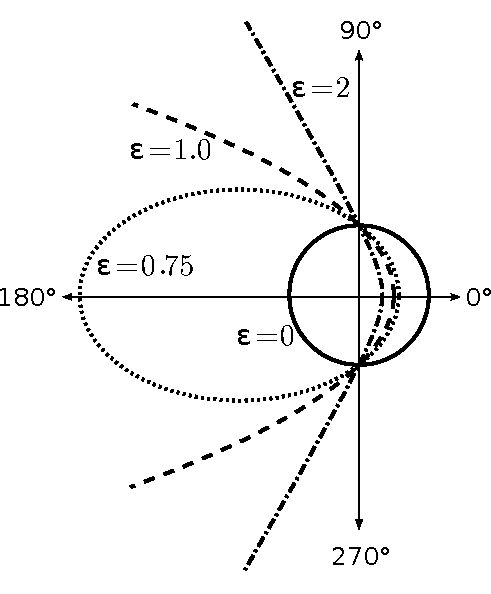
\includegraphics[width=\textwidth]{./conic_section_orbits.pdf}}
	  \end{minipage}
	  \begin{minipage}{.62\columnwidth}
		\center{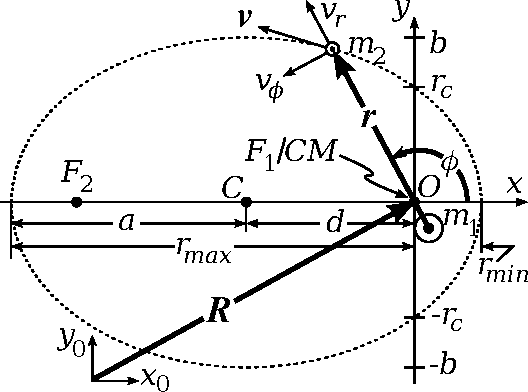
\includegraphics[width=\textwidth]{./ellipse_properties.pdf}}
	  \end{minipage}\\
		\begin{mydescription}
		  \item[Definitions:] \ \\
			$M=m_1+m_2$ \\
			$\mu=\frac{m_1m_2}{m_1+m_2}$ \\
			e.g., $U(\rho)=\frac{-Gm_1m_2}{\rho}$ \\
			$\bm{r}$: vector from body 1 to body 2 \\
			$\bm{R}$: vector from origin in inertial frame to system's CM
		  \item[Kinetic energy:] $T=\frac{1}{2}M\dot{r}^2+\frac{1}{2}\mu\dot{r}^2$
		  \item[Lagrangian:] $\mathscr{L}=\frac{1}{2}\mu\dot{\rho}^2+\frac{1}{2}\mu{\rho}^2\dot{\phi}^2-U(\rho)$
		  \item[Solution in $\phi$:] $\dot\phi=\frac{\ell}{\mu\rho^2}$ ($\ell$ const --- angular momentum)
		  \item[Solution in $\rho$:] $\mu\ddot{\rho}=-\frac{d}{d\rho}U(\rho) + \frac{\ell^2}{\mu\rho^3} = -\frac{d}{d\rho}\left[U(\rho)+\frac{\ell^2}{2\mu\rho^2}\right]$
		  \item[Effective potential:]$U_{eff}=U(\rho)+\frac{\ell^2}{2\mu\rho^2}$
		  \item[Note cons. of energy:] $\frac{d}{dt}\left( \frac{1}{2}\mu\dot\rho^2 \right) = -\frac{d}{dt}U_{eff}(\rho)$; $E=\frac{1}{2}\mu\dot\rho^2+U_{eff}(\rho)$
		  \item[Use:]$u=1/r$ and $\frac{d}{dt}=\frac{d\phi}{dt}\frac{d}{d\phi}=\dot\phi\frac{d}{d\phi}=\frac{\ell}{\mu\rho^2}\frac{d}{d\phi}=\frac{\ell u^2}{\mu}\frac{d}{d\phi}$
		  \item[$u$-equation:]$u''(\phi)=-u(\phi)-\frac{\mu}{\ell^2u(\phi)^2F(u)}$
		  \item[Use:]$\gamma=Gm_1m_2$ and $F(u)=-\gamma u^2$; then $U''(\phi)=-u(\phi)+\gamma\mu/\ell^2$; use $w(\phi)=u(\phi)-\gamma\mu/\ell^2$, so $W(\phi)=A\cos(\phi-\delta)$ ergo $u(\phi)=\frac{\gamma\mu}{\ell^2}+A\cos\phi$
		  \item[Radial eqn:] $r(\phi)=\frac{r_c}{1+\varepsilon\cos\phi}$
		  \item[Cartesian:] $\left( \frac{x+\frac{r_c\varepsilon}{1-\varepsilon^2}}{\frac{r_c}{1-\varepsilon^2}} \right)^2+\left( \frac{y}{\frac{r_c}{\sqrt{1-\varepsilon^2}}} \right)^2 = 1$
		  \item[Eccentricity:] $\varepsilon=A\cdot r_c$ ($A$ some constant)
		  \item[Circular orbit:] $r_c=\ell^2/\gamma\mu$
		  \item[Min radius:] $r_{min}=\frac{r_c}{1+\varepsilon}=\frac{\ell^2}{\gamma\mu(1+\varepsilon)}$ (at $\phi=0$; \textbf{periapsis}); $\ell=\mu rv_{tan}$
		  \item[Max radius:] $r_{max}=\frac{r_c}{1-\varepsilon}$ (at $\phi=\pi$; \textbf{apoapsis})
		  \item[Radial ($\hat r$) velocity:]$v_r = \sqrt{\frac{\mu}{r_c}}\cdot\varepsilon\cdot\sin\phi$
		  \item[Tangential ($\hat\phi$) velocity:]$v_\phi = \sqrt{\frac{\mu}{r_c}}\cdot\left(1+\varepsilon\cdot\cos\phi\right)$
		  \item[Ellipse params:] $a=\frac{r_c}{1-\varepsilon^2}$; $b=\frac{r_c}{\sqrt{1-\varepsilon^2}}$; $d=a\varepsilon$; $\varepsilon=\sqrt{1-(b/a)^2}$
		  \item[Orbital period:] $\tau=2\pi\sqrt{\frac{a^3}{\mu}}$
		  \item[Energy:] $E=\frac{\gamma^2\mu}{2\ell^2}(\varepsilon^2-1)$
		  \item[Kepler's $1^{st}$ law:] Orbits: ellipses w/ sun at a focus (approx. true)
		  \item[Kepler's $2^{nd}$ law:] Line from Sun to planet, const. area/time\\
			$dA=\frac{1}{2}r^2d\phi$; $\frac{dA}{dt}=\frac{1}{2}\frac{\ell}{\mu}$, inep. of time
		  \item[Kepler's $3^{rd}$ law:] $\tau=\frac{A}{dA/dt}=\frac{2\pi ab\mu}{\ell} \Rightarrow \tau^2=4\pi^2\frac{a^3r_c\mu^2}{\ell^2}=4\pi^2\frac{a^3\mu}{\gamma}\approx \frac{4\pi^2}{GM_s}a^3$
		\end{mydescription}

	\subsection*{Coupled oscillators}
		\begin{mydescription}
		  \item[] $\bm{M\ddot x = -Kx}$, \hspace{5pt} with
			$(\bm{M,K})\in\mathbb{R}^{N\times N}$ and
			$\bm{x}\in\mathbb{R}^{N\times 1}$
		  \item[assume solution:] $\bm{x} = \mathrm{Re}\,\left\{\bm{z}(t)\right\}$, $\bm{z}(t)=\bm{a}_ne^{i\left(\omega_nt-\delta_n\right)}$ \\
			$n \, \in \, \mathbb{Z} \: \cap \: [1,\,N]$ \\
			$\bm{a}_n\in\mathbb{R}^{N\times 1}$ = eigenvectors \\
			$\omega_n\in\mathbb{R}$ = eigenvalues \\
			$\delta_n\in\mathbb{R}$ = phase term (can be excluded, whereupon $\bm{a}_{n}\in\mathbb{C}$) \\
		  \item[actual solution:]
			$\bm{x}=\mathrm{Re}\, \left\{\sum_nA_n\bm{a}_ne^{i\left(\omega_nt-\delta_n\right)}\right\}$,
			$A_n\in\mathbb{R}$
		  \item[normal frequencies:] $\omega_n$; are the generalized eigenvalues of system
		  \item[normal modes:] solutions to equations of motion only containing
			one of the $\left\{ \omega_n \right\}$; \emph{all} motion can be
			described as a weighted sum of the normal modes; equations of
			motion written in terms of $\xi_n$ diagonalize both $\bm{M}$ and
			$\bm{K}$
		  \item[normal coordinates:] $\xi_n$; vary independently of one
			another \\
			e.g.: 2 $m$'s, 3 $k$'s, $k_1=k_3$: $\xi_1=\frac{1}{2}\left( x_1+x_2 \right)$ \&
			$\xi_2=\frac{1}{2}\left( x_1-x_2 \right)$ 
		  \item[General case:] 
		\end{mydescription}

	\subsection*{Deformable solids (linear, isotropic)}
	\textbf{Continuum hypothesis:} Matter can be treated as continuous on a large enough
	scale ($\ge\mu$m)
	\subsubsection*{Moduli}
		\begin{mydescription}
		  \item[Bulk modulus $\mathrm{BM}$:]measures substance's resistance to
			uniform compression. Defined as pressure increase needed to cause a
			given relative decrease in volume. SI unit is pascal. \\
			$\mathrm{BM} = -V\frac{\partial P}{\partial V}$
		  \item[Young's modulus $\mathrm{YM}$:] measure of stiffness of an
			isotropic elastic material. Defined as ratio of uniaxial stress
			over the uniaxial strain. SI unit is pascal. \\
			$\mathrm{YM} = \frac{F/A}{\Delta L/L}$\hspace{5pt}where $F$=force,
			$A$=area force is applied to, \& $\Delta L/L$=fractional change of
			length
		  \item[Shear modulus $\mathrm{SM}$:]deformation of a solid
			experiencing a force $||$ to one of its surfaces while its opposite
			face experiences an opposing force (such as friction). SI unit is
			pascal. \\
			$\mathrm{SM} = \frac{F/A}{\Delta x/I}$\hspace{5pt}where $F$=force,
			$A$=area force is applied to, $\Delta x$ is transverse
			displacement, \& $I$=initial length
		  \item[Poisson's ratio $\nu$:]ratio, when a sample object is
			stretched, of the contraction or transverse strain (perpendicular
			to the applied load), to the extension or axial strain (in the
			direction of the applied load)\\
			$\nu=-\frac{\varepsilon_\mathrm{trans}}{\varepsilon_\mathrm{axial}}$ \\
			\hspace{10pt}$\varepsilon_{\mathrm{trans}}$=trans. strain ($-$ for axial tension, $+$ for axial compr) \\
			\hspace{10pt}$\varepsilon_{\mathrm{axial}}$=axial strain ($+$ for axial tension, $-$ for axial compr)
		  \item[Interrelationships] \ \\
			$\mathrm{YM} = 2\mathrm{SM}\left( 1+\nu \right)$ \\
			$\mathrm{YM} = 3\mathrm{BM}\left( 1-2\nu \right)$ \\
			$\mathrm{YM} = \frac{9\mathrm{BM}\cdot\mathrm{SM}}{3\mathrm{BM}+\mathrm{SM}}$
		\end{mydescription}

	\subsubsection*{Wave equation in taut string}
		\[ \frac{\partial^2u}{\partial t^2} = c^2 \frac{\partial^2u}{\partial x^2} \] \\
		\textbf{Definitions} \\
		\hspace{10pt}$c=\sqrt{T/\mu}=$ speed of propagation \\
		\hspace{10pt}$T=$ tension \\
		\hspace{10pt}$\mu=$ linear density \\
		\hspace{10pt}$k=\omega/c=2\pi/\lambda=n\pi/L$ (for finite string) $=$ wave number, $n\ge 1$ \\
		\hspace{10pt}$\omega=2\pi c/\lambda=n\pi c/L$ (for finite string) $=$ circ. freq \\
		\hspace{10pt}$\nu=c/\lambda=nc/2L$ (for finite string) $=$ ang. freq
		\begin{mydescription}
		  \item[Infinitely-long string] \ \\
			  \textit{General sol'n}: Wave $f$ moving ($\rightarrow$) \& wave $g$ moving ($\leftarrow$) \\
			$u(x,t) = f(x-ct) + g(x+ct)$\\
			$\frac{\partial u}{\partial t} = -cf'(x-ct) + cg'(x+ct)$\\
			  \textit{Standing waves}: $u(x,t)=A\sin(kx-\omega t)+ A\sin(kx+\omega t)=2A\sin(kx)\cos(\omega t)$
		  \item[Finite string] \ \\
			  $u(x,t)=\sum_{n=1}^{\infty} \sin k_nx\left( B_n \cos\omega_n t + C_n \sin \omega_n t \right)$ \\
			  \vspace{5pt}
			  \hspace{-5pt}\textit{Solve for initial conditions:} \\
			  \vspace{2.5pt}
			  $u(x,0)=\sum_{n=1}^{\infty} B_n\sin k_nx$ \\
			  $$B_n = \frac{2}{L}\int_{0}^{L} \! u(x,0)\,sin \left(\frac{n\pi x}{L}\right) \, dx, \;\; n \geq 1$$\\
			  $\dot{u}(x,0)=\sum_{n=1}^{\infty} \omega_n C_n\sin k_nx$ \\
			  $$C_n = \frac{2}{\omega_nL}\int_{0}^{L} \! \dot{u}(x,0)\,sin \left(\frac{n\pi x}{L}\right) \, dx, \;\; n \geq 1$$\\

\end{mydescription}
   

\section*{Electromagnetics}
	\subsection*{Maxwell's equations}
    	\begin{tabular}{l l l}
			\textbf{Name} & \textbf{In general:} & \textbf{In matter:} \\
			[3pt] \\
			Coulomb & $\nabla\cdot\bm{E}=\frac{1}{\varepsilon_0}\rho$  & $\nabla\cdot\bm{D}=\rho_f$ \\
    		[3pt]
			Faraday & $\nabla\times\bm{E}=-\frac{\partial \bm{B}}{\partial t}$ & $\nabla\times\bm{E}=-\frac{\partial \bm{B}}{\partial t}$ \\
    		[3pt]
			No name & $\nabla\cdot\bm{B}=0$  & $\nabla\cdot\bm{B}=0$ \\
    		[3pt]
			Ampere+Maxwell & $\nabla\times\bm{B} = \mu_0\bm{J} + \mu_0\varepsilon_0\frac{\partial \bm{E}}{\partial t}$ & $\nabla\times\bm{H} = \bm{J}_f + \frac{\partial \bm{D}}{\partial t}$
 		\end{tabular}

	\subsection*{Boundary conditions}
    	\begin{tabular}{l l}
			\textbf{Electric} & \textbf{Magnetic} \\
			$\varepsilon_1E_1^\perp-\varepsilon_2E_2^\perp=\sigma_{f}$ & $B_1^\perp-B_2^\perp=0$ \\
			$\bm{E}_1^\parallel-\bm{E}_2^\parallel=0$ & $\frac{1}{\mu_1}\bm{B}_1^\parallel-\frac{1}{\mu_2}\bm{B}_2^\parallel=\bm{K}_f\times\uv{n}$ \\
			%${E}_{\textrm{out}}^{\perp} - {E}_{\textrm{in}}^{\perp} = \frac{1}{\varepsilon_0} \sigma$ &
			%	${B}_{\textrm{out}}^{\perp} = {B}_{\textrm{in}}^{\perp}$ \\
			%$\bm{E}_{\textrm{out}}^{\parallel} = \bm{E}_{\textrm{in}}^{\parallel}$ &
			%	$\bm{B}_{\textrm{out}}^{\parallel} - \bm{B}_{\textrm{in}}^{\parallel} = \mu_0 K$ \\
			%${D}_{\textrm{out}}^{\perp} - {D}_{\textrm{in}}^{\perp} = \sigma_{\textrm{free}}$ &
			%	${H}_{\textrm{out}}^{\perp} - {H}_{\textrm{in}}^{\perp} = -\left( M_{\textrm{out}}^{\perp} - M_{\textrm{in}}^{\perp} \right)$ \\
			%$\bm{D}_{\textrm{out}}^{\parallel} - \bm{D}_{\textrm{in}}^{\parallel} = \bm{P}_{\textrm{out}}^{\parallel} - \bm{P}_{\textrm{in}}^{\parallel}$ &
			%	$\bm{H}_{\textrm{out}}^{\parallel} - \bm{H}_{\textrm{in}}^{\parallel} = \bm{K}_{\textrm{free}}\times \uv{n}$ \\
			$V_{\textrm{1}} = V_{\textrm{2}}$ & $\bm{A}_{\textrm{1}} = \bm{A}_{\textrm{2}}$ \\
				$\pd{V_{\textrm{1}}}{n} - \pd{V_{\textrm{2}}}{n} = -\frac{1}{\varepsilon_0}\sigma$ &
				for $\div{A}=0$, $\pd{\bm{A}_{\textrm{1}}}{n} - \pd{\bm{A}_{\textrm{2}}}{n} = -\mu_0 K$ \\
			%or $\pd{V}{n} = \grad{V}\dot\uv{n}$ &
    	\end{tabular}
	\subsection*{Maxwell stress tensor}

	\subsection*{Auxiliary fields}
    	\begin{tabular}{l l}
    		\textbf{Definitions:} & \textbf{Linear media:} \\[3pt]
    		\\[3pt]
			$\bm{D}=\varepsilon_0\bm{E}+\bm{P}$ &
			$\bm{P}=\varepsilon_0\chi_e\bm{E}\;\;$, $\;\;\bm{D}=\varepsilon\bm{E}$ \\
			$\bm{H}=\frac{1}{\mu_0}\bm{B}-\bm{M}$ &
			$\bm{M}=\chi_m\bm{H}\;\;$, $\;\;\bm{H}=\frac{1}{\mu}\bm{B}$
 		\end{tabular}
	
	\subsection*{Potentials}
		$\bm{E}=-\nabla V - \frac{\partial A}{\partial t}\;\;$, $\;\;\bm{B}=\nabla\times\bm{A}$

	\subsection*{Energy, momentum, and power}
		\begin{mydescription}
			\item[energy/work] $U = \frac{1}{2}\int\left( \varepsilon E^2+\frac{1}{\mu}B^2 \right) d\tau\;$ or $\;U = \frac{1}{2}\int\rho V d\tau$ \\
				superposition: $U_{sup} = U_1 + U_2 + \varepsilon\int\bm{E_1}\cdot\bm{E_2}$
			\item[momentum] $\bm{P} = \varepsilon\int\left( \bm{E}\times\bm{B} \right)d\tau$
			\item[Poynting vector] $\bm{S} = \frac{1}{\mu}\left( \bm{E}\times\bm{B} \right)$
			\item[Larmor formula] $P = \frac{\mu}{6\pi c}q^2a^2$
		\end{mydescription}

	\subsection*{Devices}
		\begin{mydescription}
			\item[capacitor] Holding voltage constant, $U_{\textrm{tot}} = U_{\textrm{batt}} + U_{\textrm{push}}$ \\
				$dU = VdQ + F_{\textrm{push}}dx$ \\
				$\bm{F_E} = +$<++>
			\item[electromagnet] Holding current constant, $U_{\textrm{tot}} = U_{\textrm{batt}} + U_{\textrm{push}}$; $dU = VdQ + F_{\textrm{push}}dx$ \\
		\end{mydescription}




\section*{Optics}
  \subsubsection*{Geometric}

  \subsubsection*{Diffraction}
  	
  \subsubsection*{Scattering}

  \subsubsection*{Nonlinear}

\section*{Special Relativity}
  \subsubsection*{Axioms}
		\begin{mydescription}
			\item[Principle of Relativity:] The laws by which the states of
			  physical systems undergo change are not affected, whether these
			  changes of state be referred to the one or the other of two
			  systems in uniform translatory motion relative to each other.\\
			\item[Principle of Invariant Light Speed:] Light travels at $c$
			  regardless of motion of the source of the light or the inertial
			  frame in which it is observed \\
			\item[Isotropy \& Homogeneity of Space] \ \\
			\item[Independence of Measuring Devices on their History]
		\end{mydescription}
  \subsubsection*{Consequences}
		\begin{titemize}
			\item Time dilation
			\item Lorentz (length) contraction
			\item Relativity of simultaneity
			\item Composition of velocities
			\item Inertia and momentum
			\item Equivalence of mass and energy
			%\item[Time dilation]
			%\item[Lorentz (length) contraction]
			%\item[Relativity of simultaneity]
			%\item[Composition of velocities]
			%\item[Inertia and momentum]
			%\item[Equivalence of mass and energy]
		\end{titemize}

  \subsubsection*{Lorentz transformations}
    \hspace{5pt}$t' = \gamma \left(t - vx/c^2\right)$ \\
    \hspace{5pt}$x' = \gamma \left(x - v t\right)$ \\
    \hspace{5pt}$y' = y$ \\
    \hspace{5pt}$z' = z$ \\
    \hspace{5pt}$\gamma = \frac{1}{\sqrt{1 - \left({v}/{c}\right)^2}}$
  
  \subsubsection*{Generally\dots}
	\hspace{5pt}$E^2 = {\left( pc \right)^2 + \left(mc^2\right)^2}$; $E$ is total energy of particle \\
	\hspace{5pt}$p = \frac{1}{c}\sqrt{E^2 - \left(mc^2\right)^2}$ \\
	\hspace{5pt}$\bm{p}c^2 = E\bm{v}$ \\
	\hspace{5pt}$\bm{F}=\frac{d\bm{p}}{dt}$
  \subsubsection*{Moving mass}
	\hspace{5pt}$E=\gamma mc^2$ \\
	\hspace{5pt}$\bm{p}=\gamma m \bm{v}$ \\
	\hspace{5pt}$\gamma = 1/\sqrt{1-(v/c)^2}$ \\
  \subsubsection*{Photons}
	\hspace{5pt}$E = pc$, \hspace{5pt}or $E = \hbar \omega$, \hspace{5pt} or $E = hc/\lambda$ \\
	\hspace{5pt}$\bm{p} = \hbar \bm{k} = h\nu/c = h/\lambda$ \\
	\hspace{5pt}$k=2\pi/\lambda$ \\

\section*{Quantum Mechanics}
  \subsubsection*{de Broglie}
	\hspace{5pt}for ALL things, light \& matter: \\
	\hspace{15pt}$\lambda=h/p$ \\
	\hspace{15pt}$\nu=E/h$
  \subsubsection*{Schr\"odinger Equation}
  	$$ i\hbar\frac{\partial\Psi}{\partial t} = -\frac{\hbar^2}{2m}\frac{\partial^2\Psi}{\partial x^2} + V\Psi$$
	\hspace{5pt}this is non-relativistic\\
	\hspace{5pt}$\Psi$ can be complex-valued\\
	\hspace{5pt}boundary conditions lead to energy quantization\\
	\hspace{5pt}not derived (initially) but fit to reality\\
  \subsubsection*{Time Independent Schr\"odinger Equation}
  	$$ -\frac{\hbar^2}{2m}\frac{\partial^2\psi}{\partial x^2} + V\psi = E\psi$$
  \subsubsection*{Quantum Things}
  	\begin{titemize}
  	  \item Mass, charge, etc.
	  \item Energy (cf. blackbody radiation, photoelectric effect,
		  photons \& other fields)
	  \item Interference -- 2 slit experiment
  	  \item Tunneling (radioactive decay, electronic devices)
  	  \item Zero-point motion, i.e., electron never at 0 energy 
  	  \item Diffraction in matter
  	\end{titemize}
  \subsubsection*{Operators}
  	\hspace{5pt}position, $\langle x \rangle$: $\hat{x} = x$ \\
	\hspace{5pt}a function of position, $\langle f(\bm{r})\rangle$: $\hat{f}=f(\bm{r})$ \\
	\hspace{5pt}velocity, $\langle v\rangle=\frac{d\langle x \rangle}{dt}$: $\hat{\bm{v}} = \frac{\hbar}{im}\bm\nabla$ \\
	\hspace{10pt}Note that this is velocity of expectation, but gives velocity in QM\\
	\hspace{5pt}momentum, $m\frac{d\langle x \rangle}{dt}$: $\hat{\bm{p}}=\frac{\hbar}{i}\bm\nabla$ \\
	\hspace{5pt}energy: $\hat H = -\frac{\hbar^2}{2m}\bm\nabla^2+V$

\section*{Waves}
  \subsubsection*{Forms}
	  $$ \bm\nabla^2 \bm A = \frac{1}{v^2} \frac{\partial^2 \bm A}{\partial t^2} $$
	For any $f(x)$, $f(x\pm vt)$ is a traveling wave and solves the wave eqn.\\
	$\sin\frac{2\pi}{\lambda}\left( x-vt \right) =
		\sin\left( \frac{2\pi}{\lambda}x \pm \frac{2\pi}{T}t \right) =
		\sin\left( \frac{2\pi}{\lambda}x \pm 2\pi f t \right) = 
		\sin\left( kx\pm \omega t \right)$
  \subsubsection*{Simple Diffraction}
	  \hspace{5pt}$\sin\theta = n\lambda/2\pi$

\section*{Thermodynamics \& Statistical Mechanics}
  \subsubsection*{Fundamentals}
    \textbf{0$^{th}$ Law}---If sys $A$ in therm eqlib w/ sys $B$ \& $B$
    	in therm eqlib w/ sys $C$, $A$ in eqlib w/ $C$ \\
    	\textbf{1$^{st}$ Law}---Cons. of energy; $\Delta U_{tot} = Q+W_{tot}$ \\
    \textbf{2$^{nd}$ Law}---$S_{tot}$ for an isolated sytem always stays
    	the same or increases \\
    \textbf{3$^{rd}$ Law}---As $T \rightarrow 0$, $S \rightarrow 0$; OR as
    	$T\rightarrow0$, $C_V\rightarrow0$ \\
    \textbf{Fundamental Assumption of Stat Mech}---Given an isolated system
    	in equilibrium, it is found with equal probability in each of its
    	accessible microstates \\
  \subsubsection*{Definitions}
  \textbf{Random walk} $\langle \vec{L}\rangle =0$ $\sqrt{\langle \vec{L}^2\rangle}=\ell\sqrt{N}$, independent of number of dimensions \\
  mean free path: $\ell\approx \frac{1}{4\pi r^2}\frac{V}{N}$ \\
  time between collisions: $\langle \Delta t\rangle\approx \frac{\ell}{v_{\textrm{rms}}}$ \\
    \textbf{Temperature}---$T\equiv \left( \frac{\partial S}{\partial U} \right)^{-1}$\\
    1. Measure of the tendency of an object to spontaneously give up energy to
      its surroundings. \\
    2. That which is the same for two systems in thermal equilibrium. \\
    \emph{NOTE} A negative temperature is \emph{hotter} than an infinite
    temperature. \\
	\vspace{2.5pt}
  \textbf{Heat}---Any spontaneous flow of energy from one object to another
    caused by a difference in temp between the objects. \\
	\emph{Mechanisms}: conduction, convection, radiation \\
	\vspace{2.5pt}
  \textbf{Work}---Any other transfer of energy into or out of a system.\\
    \hspace{5pt}\emph{quasistatic compression}:
    $W=-P\Delta V = -\int_{V_i}^{V_f}P(V)\:\textrm{d}V$ \\
  \vspace{2.5pt}
	\textbf{Heat Capacity}---Heat required to increase the temp of a substance \\
	  \hspace{5pt} $\mathbb{C} \equiv \frac{Q}{\Delta T}$\\
	  \hspace{5pt} specific heat capacity: $c = \frac{Q}{m \Delta T} = \frac{\mathbb{C}}{m}$\\
	  \hspace{5pt} $\mathbb{C}_V = \left( \frac{\partial U}{\partial T} \right)_{V,N}$
	    (since $Q=\Delta U-W$ and $W=-P\Delta V$); ``energy capacity''\\
		\hspace{5pt} $\mathbb{C}_{P} = \left( \frac{\partial U + P\partial V}{\partial T} \right)_{P,N} = \left( \frac{\partial H}{\partial T} \right)_{P,N}$; ``enthalpy capacity''\\
  \vspace{2.5pt}
  \textbf{Latent Heat}---For a phase transition (1$^{st}$-order), energy goes
    into / comes out of molecular rearrangement, \emph{not} a change in KE, so $Q
	\nRightarrow \Delta U$, and $\mathbb{C}\rightarrow \infty$. \\
	\hspace{5pt} $L \equiv \frac{Q}{m}$ \\
  \vspace{2.5pt}
  \textbf{Entropy}---$S \equiv k_B\ln \Omega$; SI units of J/K \\
    \hspace{5pt} $\Delta S = \Delta U/T = Q/T$ (const. temp \& vol, no work)\\
	\hspace{5pt} $dS = Q/T =\frac{C_VdT}{T} \Rightarrow \Delta S = S_f-S_i = \int_{T_i}^{T_f}\frac{Q}{T}dT = \int_{T_i}^{T_f} \frac{C_V}{T}dT$ ($V$ const, $W$=0, $T$ varying)\\
	\hspace{5pt} or $\Delta S = \int_{T_i}^{T_f}\frac{Q}{T}dT$ if $W\ne0$

	\hspace{5pt} Mixing \emph{different} gasses: $\Delta S_{A}=N_{A}\ln(V_{f,A}/V_{i,A})$; $\Delta S_{tot} = \Delta S_A + \Delta S_B$ \\

    \hspace{5pt} Einstein solid, high-T: $S \approx Nk_B\ln U - Nk_B\ln (\epsilon N) + Nk_B$ \\
	\hspace{5pt} Monatomic ideal gas: $S \approx Nk_B\ln V + NK\ln U^{3/2} + f(N)$ \\
  \vspace{2.5pt}
  \textbf{Enthalpy}---$H$; $\Delta H$ is equal to the change in the internal
    energy of the system, plus the work that the system has done on its
    surroundings. \\
	\hspace{5pt}$H \equiv U + P \mathrm{d}V$ \\
	\hspace{5pt}$\Delta H = \Delta U + P \Delta V + W_{non-compr/exp}$ \\
	\hspace{5pt}If $P$ is const., $\Delta H = Q + W_{non-compr/exp}$ \\
  \vspace{2.5pt}
  \textbf{Gibbs Free Energy}---$G \equiv U+PV-TS = H-TS$ \\
    \hspace{5pt}Energy $TS$ into rabbit from surroundings; extra energy $PV$ to displace atmosphere \\
  \vspace{2.5pt}
  \textbf{Helmholtz Free Energy}---$F \equiv U - TS$ \\
    \hspace{5pt} Energy $TS$ into rabbit from surroundings; NO accounting for $PV$ to displace atmosphere \\
    \hspace{5pt}$ F = -k_BT \ln Z $\\
    \hspace{5pt}$ S = - \left( \frac{\partial F}{\partial T} \right)_{V,N} $\\
    \hspace{5pt}$ P = - \left( \frac{\partial F}{\partial V} \right)_{T,N} $\\
    \hspace{5pt}$ \mu = + \left( \frac{\partial F}{\partial N} \right)_{T,V} $\\
    \vspace{2.5pt}
	\textbf{Chemical potential}---$\mu\equiv\left( \frac{\partial E}{\partial N} \right)_{S,V}$ \\
    \hspace{5pt}Change in energy with addition of a particle, other vars fixed \\
	\hspace{5pt}$\mu=\left( \frac{\partial E}{\partial N} \right)_{S,V}$ \\
	\hspace{5pt}$\mu=-T\left( \frac{\partial S}{\partial N} \right)_{U,V}$ \\
    \hspace{5pt}$\mu =\left( \frac{\partial F}{\partial N} \right)_{T,V} $\\
    \hspace{5pt}$\mu =-kT \ln \left( Z_1/N \right)$ for single-particle-state $Z$\\

  \textbf{Ideal Gas}---No interaction among particles, random motion \\
    \hspace{5pt}$PV=Nk_{B}T$ \\
	\hspace{5pt}mean translational velocity$= \sqrt{\frac{6}{5}\frac{U}{mN}}$ \\
  	\hspace{5pt}Note that \emph{non}-ideal gas yields reduced pressure due to interactions\\
  \subsubsection*{Equipartition Theorem}
    $U_{\textrm{therm}}=Nf\frac{1}{2}k_BT$ \\
    Thermal energy distributes evenly to each quadratic degree of freedom
    (true even for relativistic systems, but \emph{not} true for
    quantum-dominated systems). \\
    \textbf{Diatomic gas at low temp} has 3 DOF (3 transl) \\
    \textbf{Diatomic gas at room temp} has 5 DOF (3 transl + 2 rot) \\
    \textbf{Diatomic gas at high temp} has 5 DOF (3 transl + 2 rot + 2 vibr) \\
    \textbf{Einstein solid} has 6 DOF (3 springs = 3$\times$(1 PE + 1 KE)) \\
    \textbf{Liquid} has 3 quad DOF and other DOF non-quadratic \\
  \subsubsection*{Sackur-Tetrode equation}
    $S=NK\left[ ln\left( \frac{V}{N}\left( \frac{4\pi mU}{3Nh^2} \right)^{3/2} \right)+\frac{5}{2} \right]$ (Valid for ideal, monatomic gas)
  \subsubsection*{Isothermal Compression/Expansion} (Quasistatic)
    $\Delta T = 0$, or $T = const.$; slow heat exchange w/ outside equalizes temp\\
	$\Rightarrow \Delta U = 0$\\
	$\Rightarrow Q = -W$\\
	For ideal gas:\\
	\hspace{5pt}$P = \frac{const.}{V}$, where $const. = Nk_BT$\\
	\hspace{5pt}$W = -\int_{V_i}^{V_f}PdV = -\int_{V_i}^{V_f}Nk_BT/V\;dV = -Nk_BT \ln (Vf/Vi)$\\
	\hspace{5pt}$\Rightarrow W>0\;$ if $\;V_i > V_f$\\
	\hspace{5pt}$\Rightarrow W<0\;$ if $\;V_i < V_f$\\
  \subsubsection*{Adiabatic Compression/Expansion} (Quasistatic)
    $Q=0$ (Isolated system can't exchange heat)\\
	$\Rightarrow \Delta U = W$\\
	For ideal gas:\\
	\hspace{5pt}$\Delta U = -P \Delta V$ \\
	\hspace{5pt}$Nf\frac{1}{2}k_BdT = -P \Delta V$; since $P=Nk_BV/T\;$, $\;Nf\frac{1}{2}k_BdT = -\frac{Nk_BT}{V}dT$\\
	\hspace{5pt}$T^{f/2}V=const.$\\
	\hspace{5pt}$PV^{(f+2)/f}=const.$\\
	\hspace{5pt}Define $\gamma = (f+2)/f$, and $PV^\gamma=const.$
  \subsubsection*{Heat Conduction Law (Fourier)} 
  Generally: $Q = -k \nabla T$ \\
  One dimension: $Q_x = -k \frac{dT}{dx}$ \\
  One dimensional heat equation: $\frac{\partial T}{\partial t}= K \frac{\partial^2 T}{\partial x^2}$ with $K=\frac{k_t}{c\rho}$; \\
  $k_t=$therm conductivity, $\rho=$density, and $c=$specific heat capacity\\
  Solution to heat eqn: $T(x,t) = T_0 + \frac{A}{\sqrt{t}}e^{-x^2/4Kt}$, $A=const.$
  \subsubsection*{Probabilities and Multiplicities} 
  \textbf{Combinations:} \\
  \textbf{$N$ coins, multiplicity of macrostate with $n$ heads:}\\
	\hspace{5pt}$\Omega(N,n)=\frac{N!}{n!(N-n)!}= comb(N,n)$ \\
	\textbf{Einstein solid w/ $N$ osc ($N/3$ atoms) and $q$ units of energy ($hf$):} \\
	\hspace{5pt} $\Omega(N,q)=\frac{(q+N-1)!}{q!(N-1)!} = comb(q+N-1, q)$ \\
	\textbf{2 Einstein solids w/ $N_A$, $N_B$, and $q_{tot}$:} \\
	\hspace{5pt} Solid $A$ can have $q_A \in [0,\,q_{tot}]\Longrightarrow q_{tot}+1$ different energy levels \\
	\hspace{5pt} Solid $B$ has $q_B=q_{tot}-q_A$ energy \\
	\hspace{5pt} Multiplicity for a given macrostate (def'd by $q_A$): $\Omega_{tot} = \Omega_A \Omega_B$ \\
	\hspace{5pt} Total microstates: $\Omega_{\textrm{grand}}=\textrm{comb}(N_A+N_B+q_{tot}-1,\;q_{tot})$ \\
	\hspace{5pt} Prob of microstate: $\mathbb{P} = \Omega_{tot}/\Omega_{grand}$ \\
	\hspace{5pt} Most prob. microstate: ${q_A} = \frac{N_A}{N_A+N_B}q_{tot}$ \\
	%\textbf{For $|x| \ll 1$, $\ln (1+x) \approx x$} \\

	\textbf{Multipicities under various approximations:} \\
	\hspace{5pt} \emph{Einstein solid, large \& high temp ($N\gg 1$; $q\gg N$):} \\
	\hspace{10pt} $\Omega(N,q) \approx \left( \frac{eq}{N} \right)^N$ \\
	\hspace{5pt} \emph{Einstein solid, large \& low(er) temp ($N\gg 1$; $q\gg 1$):} \\
	\hspace{10pt} $\Omega(N,q) \approx \left( \frac{eN}{q} \right)^q$ \\
	\hspace{5pt} \emph{Einstein solid any large $N$ and $q$:} \\
	\hspace{10pt} $\Omega(N,q) \approx \frac{\left( \frac{q+N}{q} \right)^q \left( \frac{q+N}{N} \right)^N}{\sqrt{2\pi q\left( q+N \right)/N}}\approx \left( \frac{q+N}{q} \right)^q \left( \frac{q+N}{N} \right)^N$ \\
	\hspace{5pt} \emph{2 Einstein solids, large \& high temp:} \\
	\hspace{10pt} $\Omega_{tot} \approx \left( \frac{eq_A}{N_A} \right)^{N_A} \left( \frac{eq_B}{N_B} \right)^{N_B}$; if $N_A = N_B$,  $\Omega_{tot} \approx (e/N)^{2N}(q_A q_B)^N$\\
	\hspace{5pt} \emph{2-state paramagnet, large ($N_{\uparrow} \ll N$):} \\
	\hspace{10pt} $\Omega(N,N_{\uparrow}) \approx \left( \frac{eN}{N_{\uparrow}} \right)^{N_{\uparrow}}$ \\
	\hspace{5pt} \emph{Ideal Gas, $d$-Dimensional:} \\
	\hspace{10pt} $\Omega_N = \frac{1}{N!} \frac{L^{dN}}{h^{dN}} \frac{2\pi^{dN/2}}{\left( dN/2 - 1 \right)!} \left( 2mU \right)^{\left( dN-1 \right)/2}$ \\
	\hspace{10pt} ($d$=\# dimensions, $L$=length)  \\
	\hspace{5pt} \emph{Ideal Gas, 3D:} \\
	\hspace{10pt} $\Omega_N \approx \frac{1}{N!} \frac{V^{N}}{h^{dN}} \frac{\pi^{3N/2}}{\left( 3N/2 \right)!} \left( 2mU \right)^{3N/2}$ \\
	\hspace{10pt} $\Omega(U,V,N) \approx f(N) V^N U^{3N/2}$ \\
	\textbf{Sharpness of multiplicity function:} \\
	\hspace{10pt}Let $q_A = q/2 + x$, where $x$ is the offset from the midpoint\dots \\
	\vspace{2.5pt}
	\hspace{5pt} \emph{2 large Einstein solids, high temp; $N_A=N_B$} \\
	\hspace{10pt} $\Omega = \left( \frac{e}{N} \right)^{2N}e^{N\ln\left( q/2 \right)^2}-N\left( 2x/q \right)^2$ \\
	\hspace{10pt} $\Omega = \Omega_{\textrm{max}}e^{-N\left( 2x/q \right)^2}$ \\
	\hspace{10pt} $\Omega$ drops to $\Omega_{\textrm{max}}/e$ at $x = \pm\frac{q}{2\sqrt{N}}$ \\
	\hspace{10pt} so width $=\frac{q}{\sqrt{N}}$ \\
	\hspace{5pt} \emph{2 ideal gasses; $N_A=N_B=N\gg 1$} \\
	\hspace{10pt} $\Omega_{\textrm{tot}} = \left[ f(N) \right]^2\left( V_AV_B \right)^N\left( U_AU_B \right)^{3N/2}$ \\
	\hspace{10pt} width of distr. in avg energy is $\frac{U_{\textrm{tot}}}{\sqrt{3N/2}}$ \\
	\hspace{10pt} width of distr. in avg velocity is $\frac{V_{\textrm{tot}}}{\sqrt{N}}$ \\




	\textbf{Boltzmann Statistics:} \\
	\hspace{5pt} $\mathbb{P}(\textrm{state}=s) = \frac{1}{Z}e^{-E(s)/k_BT}$; $Z = \sum_s e^{-E(s)/k_BT}$ \\
	\hspace{5pt} $\mathbb{P}(\textrm{energy}=s) = \frac{1}{Z}g(s)e^{-E(s)/k_BT}$; $Z = \sum_s g(s)e^{-E(s)/k_BT}$ ($g$=degeneracy)\\
	\hspace{5pt} For non-interacting, indistinguishable particles: $Z_tot = Z_1 \cdot Z_2 \dots Z_N$ \\
	\hspace{5pt} For non-interacting, distinguishable particles: $Z_{tot} = \frac{1}{N!}Z_1^N$ \\
	\hspace{5pt} $<E> = \frac{1}{Z}\sum_s E(s) e^{-\beta E(s)}=-\frac{1}{Z}\frac{\partial Z}{\partial\beta}$ ($\beta=1/k_BT$) \\
	\hspace{5pt} $\sigma_E = k_BT\sqrt{C/k_B}$ \\
	\hspace{5pt} Maxwell speed distribution: $D(v) = \left( \frac{m}{2\pi k_BT} \right)^{3/2} 4\pi v^2e^{-mv^2/2k_BT}$ \\
	\hspace{5pt} Note from equipartition thm, $v_{rms} = \sqrt{3k_BT/m}$ for ideal gas \\
	\hspace{5pt} From Maxwell, $<v> = \sqrt{8k_BT/\pi m}$ for ideal gas \\

	\subsection*{Thermodynamic interactions}
	\textbf{Thermodynamic identity:} $dU = T \:dS - P \:dV + \mu \: dN$ (any
	  large system) \\
	  Simplifies to 1$^{st}$ law if $\Delta V$ is quasi-static, no other forms
	  of work are done, and no other relevant variables are changed.\\
		\begin{tabular}{l l l l}
		  \textbf{Interaction}& \textbf{Exchanges} & \textbf{Governed by}& \textbf{Formula} \\[1pt]
			therm       & energy, $U$ & temp, $T$           & $\frac{1}{T}=\left( \frac{\partial S}{\partial U} \right)_{V,N}$ \\
			[1pt]
			mech       & volume, $V$ & pressure, $P$       & $\frac{P}{T}=\left( \frac{\partial S}{\partial V} \right)_{U,N}$ \\
			[1pt]
			diffusive       & particles, $N$ & chem pot, $\mu$  & $\frac{\mu}{T}=-\left( \frac{\partial S}{\partial N} \right)_{U,V}$
		\end{tabular}
	\subsection*{Heat engines, heat pumps, \& refrigerators}
	\textbf{Heat engine:} \\
	  \begin{minipage}{\columnwidth}
		\center{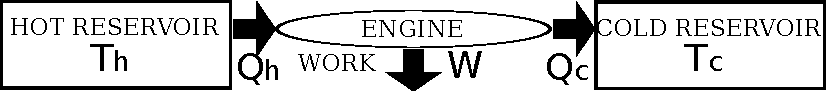
\includegraphics[width=1\textwidth]{./heat_engine.pdf}}
	  \end{minipage}\\
	\hspace{5pt} Efficiency: $e \equiv \frac{\textrm{benefit}}{\textrm{cost}} = \frac{W}{Q_h}$ \\
	\hspace{5pt} since it's a \emph{cycle}, $Q_h = Q_c+W \Rightarrow e = 1-\frac{Q_c}{Q_h}$\\
	\hspace{5pt} in terms of temp, since 2$^{nd}$ law says $\frac{Q_c}{T_c} \geq \frac{Q_h}{T_h}$, $e \leq 1-\frac{T_c}{T_h}$\\
	\textbf{Refrigerator:} \\
	  \begin{minipage}{\columnwidth}
		\center{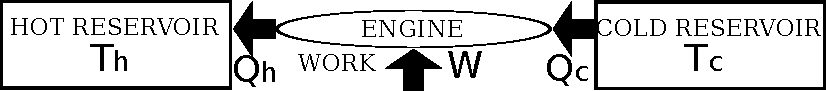
\includegraphics[width=1\textwidth]{./refrigerator.pdf}}
	  \end{minipage}\\
	\hspace{5pt} Efficiency (Coefficient of Performance): $\textrm{COP} \equiv \frac{\textrm{benefit}}{\textrm{cost}} = \frac{Q_c}{W}$ \\
	\hspace{5pt} since it's a \emph{cycle}, $Q_h = Q_c+W \Rightarrow \textrm{COP} = \frac{1}{Q_h/Q_c-1}$\\
	\hspace{5pt} in terms of temp, since 2$^{nd}$ law says $\frac{Q_h}{T_h} \geq \frac{Q_c}{T_c}$, $\textrm{COP} \leq \frac{T_c}{T_h-T_c}$\\
	\begin{minipage}{\columnwidth}
		\textbf{Carnot Cycle} \\
	%\begin{figure*}[h]
	  \begin{minipage}{0.24\columnwidth}
		\center{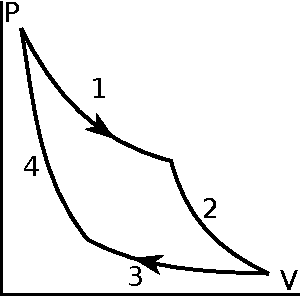
\includegraphics[width=1\textwidth]{./heat_engine_carnot_cycle.pdf}}
	  \end{minipage}\hspace{.01\columnwidth}
	  \begin{minipage}{0.74\columnwidth}
		  \begin{titemize}
			  \item[1)] isothermal expansion at $T_h$ taking in $Q_h$
			  \item[2)] adiabatic expansion to $T_c$
			  \item[3)] isothermal compression at $T_c$ expelling $Q_c$
			  \item[4)] adiabatic compression to $T_h$
		  \end{titemize}
		$e = 1-\frac{T_c}{T_h}$ \\
		Note: $S$ const for quasi-static adiabatic and isothermal processes
	  \end{minipage}\\
	\end{minipage}
	  \vspace{5pt}
	  \begin{minipage}{\columnwidth}
	\textbf{Otto Cycle} \\
	  \begin{minipage}{0.24\columnwidth}
		\center{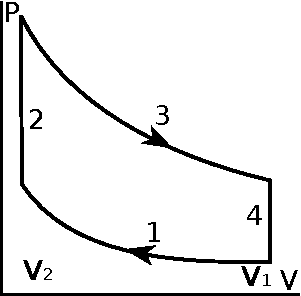
\includegraphics[width=1\textwidth]{./heat_engine_otto_cycle.pdf}}
	  \end{minipage}\hspace{.01\columnwidth}
	  \begin{minipage}{0.74\columnwidth}
		  \begin{titemize}
			  \item[1)] \emph{compression}: adiabatic compr of gas+fuel in piston\\
			  \item[2)] \emph{ignition}: fuel ignited while piston static ($V$ const; $T$ \& $P$ incr)\\
			  \item[3)] \emph{power}: adiabatic exp of gas in cylinder does work \\
			  \item[4)] \emph{exhaust}: hot gasses replaced by lower $P$, lower $T$ gas ($V$ const); fuel injected \\
		  \end{titemize}
		  \vspace{-10pt}
		{$eff = 1-\left( \frac{V_2}{V_1}\right) ^{\gamma-1} = 1 - \frac{T_1}{T_2} = 1 - \frac{T_4}{T_3}$} where $\gamma=(f+2)/f$ \\
	  \end{minipage}
	  \end{minipage}\\
	  \vspace{5pt}
	  \begin{minipage}{\columnwidth}
	\textbf{Diesel Cycle} \\
	  \begin{minipage}{0.24\columnwidth}
		\center{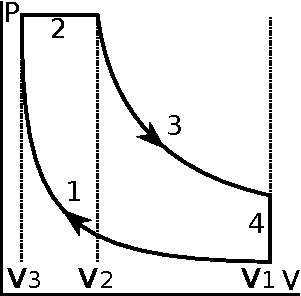
\includegraphics[width=1\textwidth]{./heat_engine_diesel_cycle.pdf}}
	  \end{minipage}\hspace{.01\columnwidth}
	  \begin{minipage}{0.74\columnwidth}
		  \begin{titemize}
			  \item[1)] \emph{compression}: (isentropic) compression of gas in
				  piston
			  \item[2)] \emph{injection/ignition}: fuel injected \& ignites;
				  $P$ const while $V\uparrow$ \& (piston moves)
			  \item[3)] \emph{expansion}: isentropic expansion w/ $P\downarrow$
			  \item[4)] \emph{exhaust}: hot gasses replaced by lower $P$, lower
				  $T$ gas ($V$ const)
		\end{titemize}
		$e=1-\frac{1}{r^{\gamma-1}}\left ( \frac{\alpha^{\gamma}-1}{\gamma(\alpha-1)} \right )$ \\
		$r=V_1/V_2$=compr. ratio; $\alpha=V_3/V_2$=cut-off ratio
	  \end{minipage}
  \end{minipage}\\

	\subsection*{Paramagnets}
	\subsubsection*{Energy}
	$U = \mu B(N_{\downarrow}-N_\uparrow) = \mu B(N-2N_\uparrow) = N\mu B \tanh(\mu B/k_BT)$
	\subsubsection*{Magnetization}
	$M = mu(N_\uparrow-N_\downarrow)=-U/B = N\mu \tanh(\mu B/k_BT)$
	\subsubsection*{Multiplicity \& entropy}
	  $\Omega(N_\uparrow)=\begin{pmatrix}[l]N\\N_\uparrow\end{pmatrix}=\frac{N!}{N_{\uparrow}!N_\downarrow!}$ \\
	  $S/k_B = \ln N! - \ln N_\uparrow! - \ln(N-N_\uparrow)! \approx N\ln N - N_\uparrow \ln N_\uparrow - (N-N_\uparrow)\ln(N-N_\uparrow)$ \\
	  $S = Nk_B\left[ \ln(2\cosh x)-x\tanh x \right]$, where $x=\mu B/k_BT$ \\
	  \textbf{sharpness} \\
	  $\Omega_{\textrm{max}} = \Omega(N,N/2)\approx 2^N \sqrt{2/\pi N}$ \\
	  $N_\uparrow = N/2+x$ and $N_\downarrow = N/2-x$ \\
	  $\Omega\approx 2^N \sqrt{2/\pi N} \; e^{-2x^2/N}$ \\
	  width$= \sigma = \sqrt{N/2}$

	\subsubsection*{Heat capacity}
	$C_B = \left( \frac{\partial U}{\partial T} \right)_{N,B} = Nk_B\frac{\left( \mu B / k_BT \right)^2}{\cosh^2\left( mu B/k_BT \right)}$
	\subsubsection*{Temperature}
	$\frac{1}{T} = (\frac{\partial S}{\partial U})_{N,B} = \frac{\partial N_\uparrow}{\partial U}\frac{\partial S}{\partial N_\uparrow} = -\frac{1}{2\mu B}\frac{\partial S}{\partial N_\uparrow} = \frac{k_B}{2\mu B}\ln\left( \frac{N-U/\mu B}{N+U/\mu B} \right)$ \\

  \begin{minipage}{\columnwidth}
	  \begin{minipage}{0.49\textwidth}
		\center{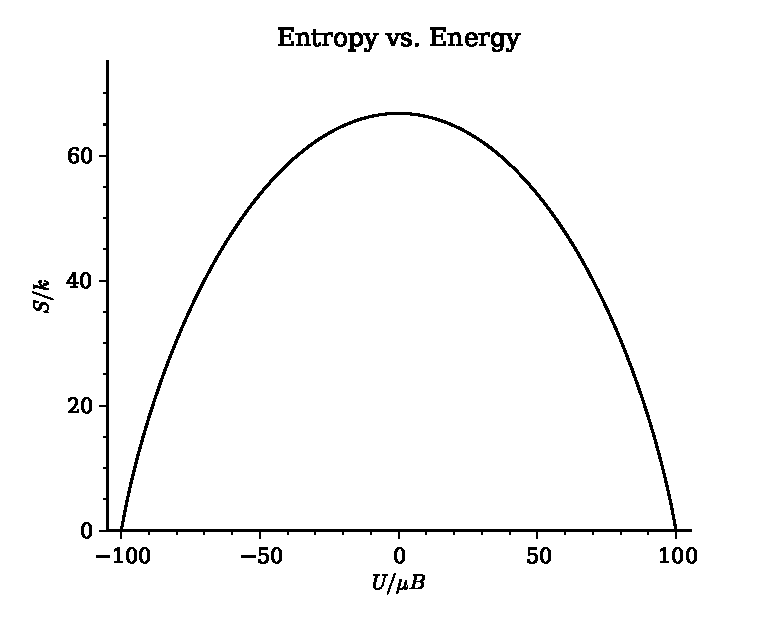
\includegraphics[width=1\textwidth]{./paramagnet_entropy_vs_energy.pdf}}
	  \end{minipage}
	  \begin{minipage}{0.49\textwidth}
		\center{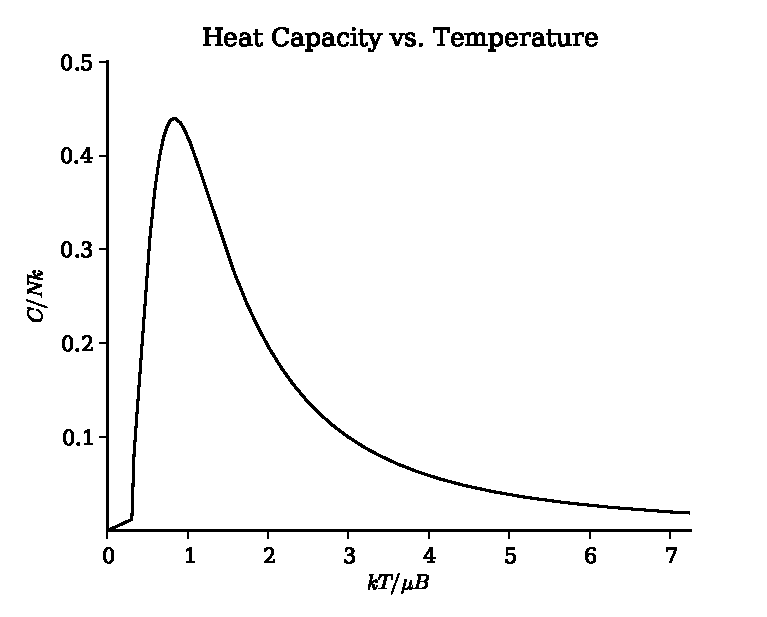
\includegraphics[width=1\textwidth]{./paramagnet_heatcap_vs_temp.pdf}}
	  \end{minipage}\\
	  \begin{minipage}{0.49\textwidth}
		\center{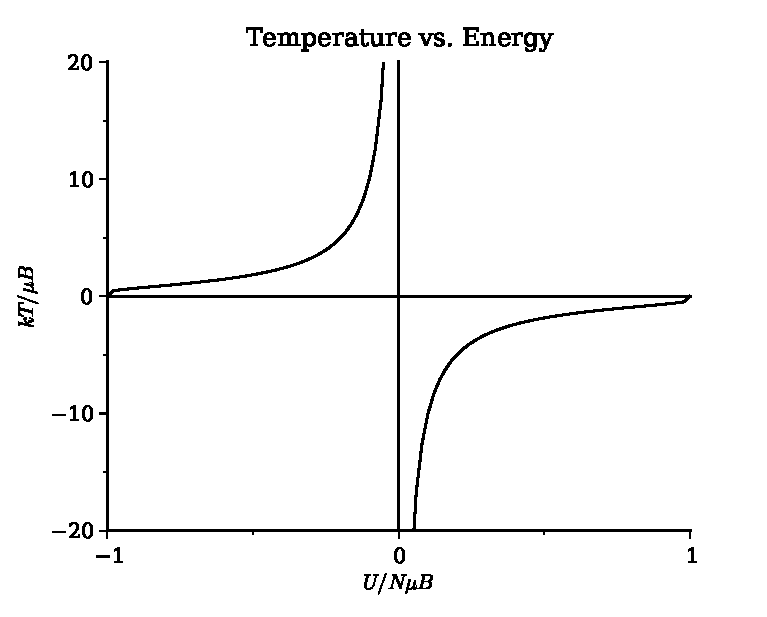
\includegraphics[width=1\textwidth]{./paramagnet_temp_vs_energy.pdf}}
	  \end{minipage}
	  \begin{minipage}{0.49\textwidth}
		\center{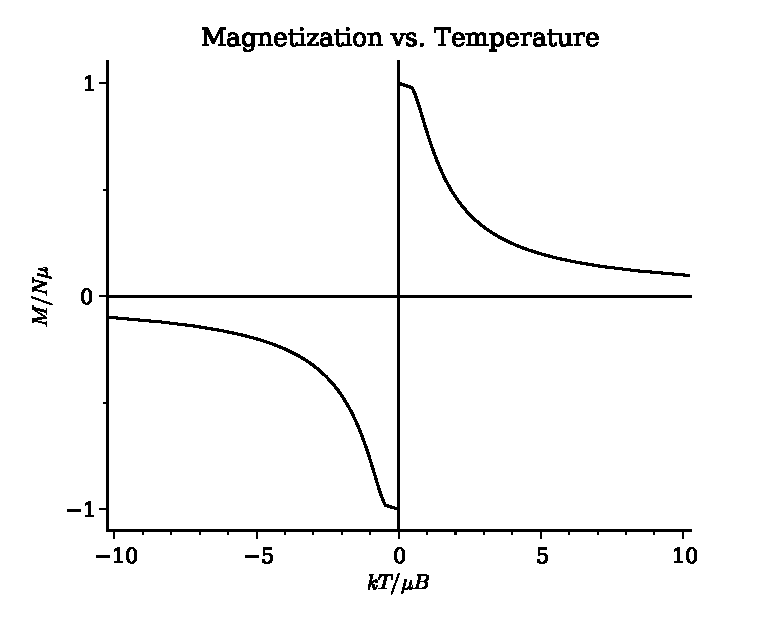
\includegraphics[width=1\textwidth]{./paramagnet_magnetization_vs_temp.pdf}}
	  \end{minipage}
  \end{minipage}


\end{multicols}
}\end{document}
